\documentclass[11pt]{article}

% preamble
\usepackage{graphicx}
\usepackage[nottoc,numbib]{tocbibind}
\usepackage{tabularx}
\usepackage[parfill]{parskip}
\usepackage{amsmath}
\usepackage[hyphens]{url}
\usepackage[hidelinks]{hyperref}
\usepackage{fancyhdr}
\usepackage{titlesec}
\usepackage{listings}
\usepackage{xcolor}
\usepackage[acronym]{glossaries}
\usepackage[all]{hypcap}
%\hypersetup{colorlinks=true, pdfstartview=FitV, linkcolor=blue, citecolor=black, plainpages=false, pdfpagelabels=true, urlcolor=blue}



\definecolor{codegreen}{rgb}{0,0.6,0}
\definecolor{codegray}{rgb}{0.5,0.5,0.5}
\definecolor{codepurple}{rgb}{0.58,0,0.82}
\definecolor{backcolour}{rgb}{1.0, 1.0, 1.0}
\lstdefinestyle{mystyle}{
    backgroundcolor=\color{backcolour},   
    commentstyle=\color{codegreen},
    keywordstyle=\color{blue},
    numberstyle=\tiny\color{codegray},
    stringstyle=\color{codepurple},
    basicstyle=\ttfamily\footnotesize,
    breakatwhitespace=false,         
    breaklines=true,                 
    captionpos=b,                    
    keepspaces=true,                 
    numbers=left,                    
    numbersep=5pt,                  
    showspaces=false,                
    showstringspaces=false,
    showtabs=false,                  
    tabsize=4
}
\lstset{style=mystyle}
\setcounter{secnumdepth}{5}

\makeglossaries

\newglossaryentry{vulkan}{name=Vulkan, description={Low-level GPU application programmable interface}}
\newglossaryentry{cpp}{name=C++,description={Low-level programming language}}
\newglossaryentry{cl}{name=CL,description={The Microsoft C compiler and linker}}
\newglossaryentry{msbuild}{name=MSBuild,description={Microsoft project build system}}

\setacronymstyle{long-short}
\newacronym{cpu}{CPU}{Central Processing Unit}
\newacronym{gpu}{GPU}{Graphics Processing Unit}
\newacronym{ram}{RAM}{Random Access Memory}
\newacronym{wsi}{WSI}{Window System Integration}
\newacronym{aes}{AES}{Advanced Encryption Standard}
\newacronym{glsl}{GLSL}{OpenGL Shading Language}
\newacronym{lib}{LIB}{Static Library}
\newacronym{dll}{DLL}{Dynamic Link Library}
\newacronym{pch}{PCH}{Precompiled Header}
\newacronym{cli}{CLI}{Command Line Interface}
\newacronym{vmve}{VMVE}{Vulkan Model Viewer and Exporter}
\newacronym{api}{API}{Application Programmable Interface}
\newacronym{exe}{EXE}{Windows Executable}
\newacronym{vma}{VMA}{Vulkan Memory Allocator}
\newacronym{ide}{IDE}{Integrated Development Environment}
\newacronym{vcs}{VCS}{Version Control System}
\newacronym{msvc}{MSVC}{Microsoft Visual Compiler}
\newacronym{stl}{STL}{C++ Standard Template Library}
\newacronym{lod}{LOD}{Level of Detail}
\newacronym{ip}{IP}{Intellectual Property}

% end of preamble

% document
\pagenumbering{gobble}

\begin{document}

\begin{titlepage}
	\centering
  
\includegraphics[scale=0.35]{images/university-logo.png}\par
  \vspace{1cm}
	{\huge\textbf{Optimizing workflow for virtual environments using Vulkan Model Viewer and Exporter}\par}
  \vspace{1cm}
  University of Roehampton\\
  Department of Arts and Digital Industries\\
  London, United Kingdom
  \vspace{1cm}
  \vfill
  \begin{minipage}[t]{0.4\textwidth}
		\begin{flushleft}
			\large
			\textit{Author}\\
			Mr. \textsc{Zakariya Oulhadj} % Your name
		\end{flushleft}
	\end{minipage}
	~
	\begin{minipage}[t]{0.4\textwidth}
		\begin{flushright}
			\large
			\textit{Supervisors}\\
			Dr. \textsc{Charles Clarke} % Supervisor's name
      \textsc{Alex Collins} % Supervisor's name
		\end{flushright}
	\end{minipage}

  \vfill
  Submitted in partial fulfillment of the requirements for the degree of \\
  \textit{Bachelors of Science in Computer Science}
  \vfill
	{\large \today\par}
\end{titlepage}

\pagebreak
\pagestyle{empty}


\begin{center}
\thispagestyle{empty}  
\vspace*{\fill}
\textit{I would like to dedicate this report to my family, friends and lecturers who have have supported me throughout my degree}
\vspace*{\fill}
\end{center}


\pagebreak

\section*{Abstract}
Computer graphics is a rapidly growing field that is vital in many industries
that rely on digital graphics including scientific research, simulations,
education and training, entertainment and more. The flexibility of this field
and the increase in computing resources is what makes it so powerful and
provides real-world benefits in ways not previously observed prior to the use of
graphics software.

This report presents my final year project \gls{vmve}, a 3D rendering
application built from the ground up using the latest technologies for virtual
environment authoring. Its goal is to be easy to use, performant and include a
collection of tools for graphics manipulation that users can take advantage of
when designing and building virtual environments.


\pagebreak

\section*{Declaration}
I hereby certify that this report constitutes my own work, that where
the language of others is used, quotation marks so indicate, and that
appropriate credit is given where I have used the language, ideas,
expressions, or writings of others. I declare that this report
describes the original work that has not been previously presented for
the award of any other degree or any other institution.

\noindent
\begin{tabular}[b]{@{} p{6cm} @{}}
\date{\today} \\
\hline
\scriptsize Date
\end{tabular}\qquad
\begin{tabular}[b]{@{} p{6cm} @{}}

\includegraphics[width=6cm,height=1cm]{images/signature.png} \\
\hline
\scriptsize Signature
\end{tabular}



\pagebreak
\tableofcontents
\addtocontents{toc}{~\hfill\textbf{Page}\par}
\pagebreak


\pagebreak

\pagestyle{fancy}
\pagenumbering{arabic}

\section{Introduction}

Computer graphics is a large area within the field of computer science. Ever
since its conception in the early 1960's it has been used for many different
purposes from gaming, the film industry, scientific research, education,
architecture, engineering, medicine and more recently within vehicles. This is a
testament to how versatile this field is.

There are many different rendering application that already exist include Unreal
Engine \cite{unreal_engine}, Unity \cite{unity} and RenderMan \cite{render_man}
just to name a few. These applications as are known as ``3D creation tools''
that provide a plethora of features and functionality giving the users the
freedom when creating digital graphics.

A common theme found within these engines as a result of being around for a
couple of decades is that they have a lot of different tools and features which
introduces their own set of issues such as  relative complexity and a steep
learning curve.

Throughout this document, I present my final year project \gls{vmve}. An
application developed in the domain of computer graphics and is a real-time 3D
rendering application designed for creating virtual environments. The aim of
\gls{vmve} is not to replicate these existing applications but instead to
purposely implement a small but specific subset of features that can be used for
common graphics related tasks. This is beneficial for a number of reasons.
Firstly, this will make \gls{vmve} easy to use as the number of features that
the user must learn is significantly reduced and subsequently lowering the
learning curve. The combination of these two benefits will make the application
far more accessible to the general public.


\subsection{Overview}
This report will discuss the projects development from beginning to end and is
is structured such that it outlines each aspect of the project in chronological
order. There are a total of five key sections to this report. The introduction,
design, implementation, evaluation and finally, future work.

The report will focus on the early stages of the project including design and
requirements gathering. The main implementation section will follow this and
provide detailed insights and technical implementation details into the project.
In order to ensure that the project has met the requirements originally set out,
an evaluation stage must undertaken. This will include discussions of various
metrics as well as reviewing the project and understanding its strengths and
shortcomings. Lastly, future work will outline additional work that needs to be
undertaken and the projects overall future.

\subsection{Aims and Objectives}
As mentioned previously, the key aim of \gls{vmve} is to implement a subset of 
specific rendering features which includes a 3D renderer, an visual editor
and lastly a custom file format for digital assets.

- Refer to milestone 2 document.
- State the problem being
addressed and why it is important to address it - large applications
consist of many requirements such as powerful hardware, applications,
steep learning curve.

- Key stakeholders


\begin{description}
  \item[Lightweight] meaning application should be highly
    efficient in regards to rendering and memory usage.
  \item[Ease of use] so that users with no prior experience
  \item[Useful]
    Another vital requirement is that it should be useful
\end{description}
  
  - Lightweight model viewer - No need to install heavy
  applications such as Blender/Unity/Unreal - Easy to use - No technical
  knowledge required


\subsection{Goals and Requirements}
In order to address these issues in this domain, a set of requirements
must be defined that aims to achieve the desired goal of this project.

Since its conception, \gls{vmve} has three main goals. The first is to provide
users with an easy to use platform that they can use for rendering digital
assets in a virtual environment. In other words, users with little to no prior
experience in computer graphics should be able to take advantage of \glspl{vmve} 
capabilities.

The second goal of the application is to 


The last out of the three main goals is for the application to include its own
model format that makes use of encryption to safely secure a users digital
assets.


\subsection{Stakeholders}
Users



\subsection{Legal}
Legal considerations are important when distributing an application indented to
be used in production. The project and subsequently the application must abide by
local laws and regulations.

\subsubsection{License}
\gls{vmve} is to be licensed under the MIT license \cite{mit}. This ensures the
application can be used without restriction allowing for it to be copied,
modified as well as distributed.

\subsubsection{Security}
Additionally, security must be taken into account when developing the
application. As mentioned earlier, \gls{vmve} will include the ability to secure
critical assets including 3D models. This will be achieved using encryption by
making use of a secret key and initialization vector.

When developing the system, it is therefore, important to ask questions such as
``How will this data be kept secure?'' and ``Does the application store or send
any private data?''. 

Throughout the development of this project, the application will not contain any
networking functionality. This ensures that all data remains local to the
application and users device.

\subsubsection{Intellectual property}
Given the application use case, it will be handling third party 3D assets such
as importing and exporting. It is therefore, important that \gls{vmve} does not
infringe upon the copyright of those who own the models. One such example
includes not modifying the geometry data unless specified by the user. Since
this will be a new application, a lot of the intricacies behind \gls{ip} needs
to be further defined and take into account based on user feedback. \gls{vmve}
will not modify any of the data being imported and only change the visual
appearance based on several factors including rendering settings, translation,
rotation and scaling. 

\subsection{Social}
\gls{vmve} must also take into account social considerations for those using the
application to provide a consistent user experience.

\subsubsection{Accessibility}
Accessibility is a vital aspect that needs to be addressed throughout the
development to ensure the application is useable for those with disabilities.

\section{Technology Review}
This project made use of various technologies at different stages throughout the
development process and was a key aspect in helping achieve the final goal of
developing a 3D model viewer and exporter.

Technologies are categorized into two areas based on the impact they have on the
project such as direct and indirect influence. A technology that has direct
impact means that it assisted in some way to the implementation of the project.
Whereas, indirect impact are technologies that are used in some areas not
directly responsible in the projects outcome such as project management.

\subsection{Tools}

\subsubsection{Project Management}
A \gls{vcs} is a tool used for backing up and/or collaborating with developers
on a project. The use of a \gls{vcs} was an obvious choice as this would provide
a platform on which the project source code could be hosted. This gives me the
peace of mind knowing that if for some reason a local copy of the project is
lost or corrupted then another copy is safely hosted on the servers managed by
the \gls{vcs}.

Another key feature of a \gls{vcs} is project management. These types of systems
provide various tools that greatly benefit developers. One such feature is known
as a ``commit'' which records any changes made to a particular repository at
that moment in time. Developers use commits to view changes that occur at each
stage but also, provides means of reverting to previous states of particular
sections, files or even an entire repository. Due to the length and complexity
of this project, tools such as this provided by \gls{vcs} are invaluable throughout
the development process.

The specific version control system that was chosen was Git \cite{gitvcs}. This
is the most popular free and open-source \gls{vcs} and is highly recommended.

Git can be used in several different ways such as installing Git onto a server
manually and interacting with Git through that server. Another way is by using
existing platforms that are built on top of Git. A few examples include GitHub,
GitLab and Bitbucket. By far the most popular option is GitHub and is the
platform that I am most familiar with.


The \gls{vmve} project is hosted on GitHub as a private repository
\url{https://github.com/ZOulhadj/vmve/}


GitHub as well as providing hosting for the repository also provides different
features related to task management. One such feature is known as GitHub issues.
This will be used as the task tracker in which ``posts'' are created that would
track outstanding tasks including the priority, current progress and the
expected deadline. Figure \ref{fig:github_kanban} shows a preview of the Kanban
board. It consists of three main columns used to categorize an issue including
backlog, in progress and done. 

When an idea for a new feature is thought of or a bug within the application is
discoverd a GitHub issue is created and moved to the ``Backlog''. This is used
to document a particular task that needs to be worked on in the near future.

Then once a specific issue is ready to be worked on/resolved, it's moved to the
``In Progress'' column. As the issue is being addressed, key points of discussion
are added as comments to the issue for documentation purposes.

Lastly, once the task has been completed, the GitHub commit that includes the
fix is referenced in the issue and is then finally marked as complete by being
moved to the ``Done'' column.

\begin{figure}[h!]
  \centering
  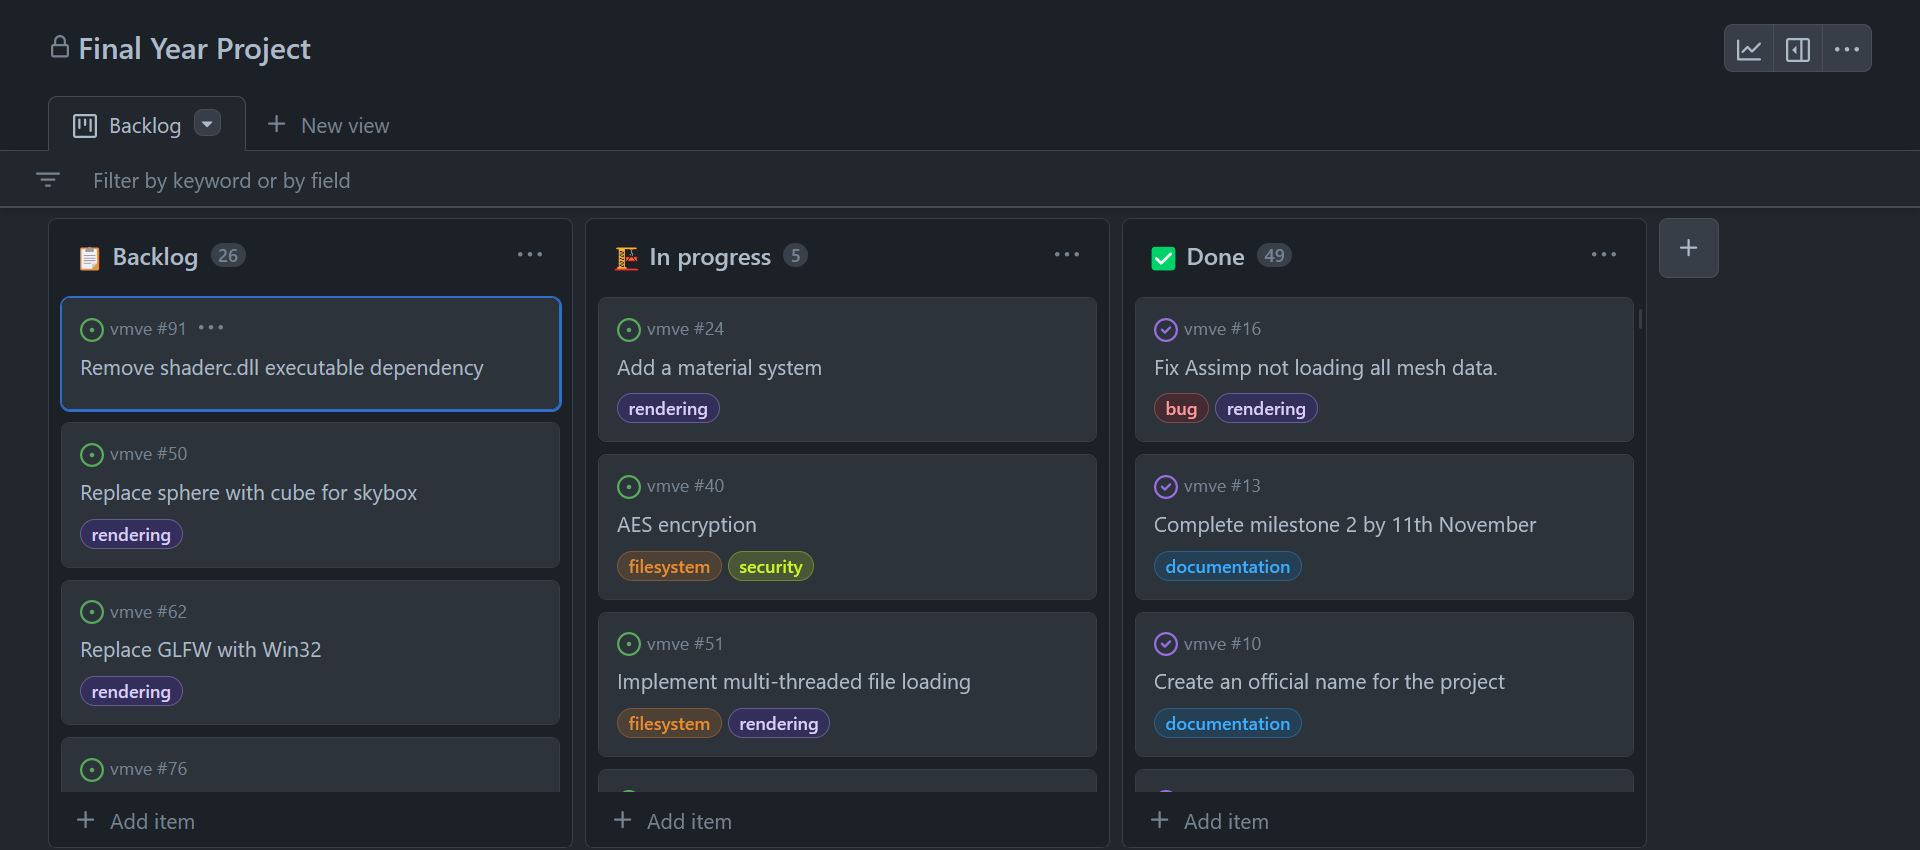
\includegraphics[width=\textwidth]{images/github_project.png}
  \caption{GitHub Issues Kanban}
  \label{fig:github_kanban}
\end{figure}

\subsubsection{Microsoft Visual Studio 2022}
Developing a program that runs directly on the underlying operating system
requires a compiler. This is a program that parses source code and generates
assembly instructions that the \gls{cpu} will be able to understand and
therefore, execute. \gls{msvc} also known as CL will be the compiler of choice.
This is a compiler that comes bundled with the Microsoft Visual Studio
\gls{ide}.

The \gls{ide} also provides debugging functionality that will be used
extensively to fix crashes, bugs and generally ensuring that the application
runs as expected \cite{visualstudio}. 

\begin{figure}[h!]
  \centering
  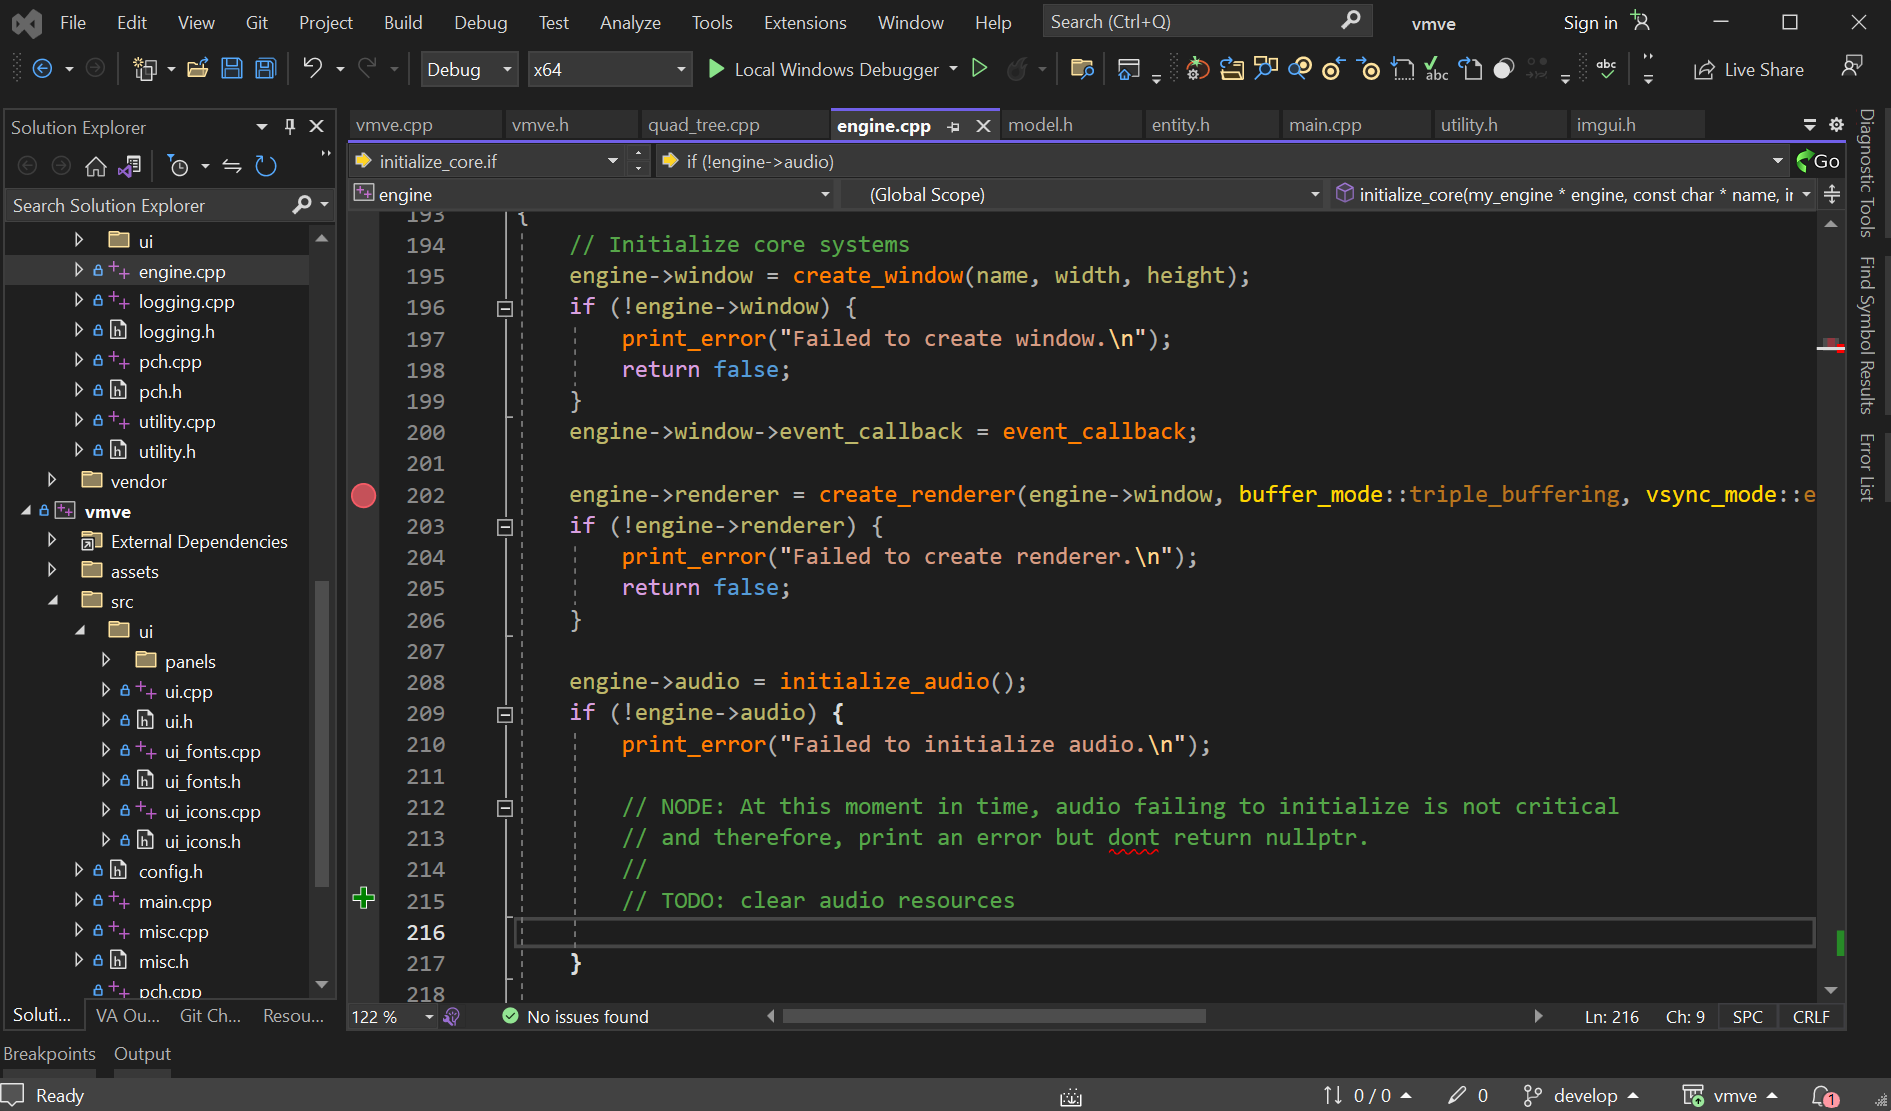
\includegraphics[width=\textwidth]{images/visual_studio.png}
  \caption{Microsoft Visual Studio}
  \label{fig:visual_studio}
\end{figure}

Some additional tools will be used that will further improve the ease of
development.  Visual Studio Assist X \cite{visualstudioassistx} is one such
tool. This is a Visual Studio extension that provides many useful features that
the based \gls{ide} does not provide such as reliable symbol renaming, file symbol
outlining, quick file searching and much more.


\subsubsection{RenderDoc}
Having discussed the various debugging tools available for \gls{cpu} debugging
there are also a couple of \gls{gpu} tools that allows for analyzing per frame
data as well as detailed frame synchronization metrics.

On such tool is called RenderDoc \cite{renderdoc} and is used to inspect
individual frames including its entire state and ensures that you can debug
particular \gls{gpu} related bugs.

\begin{figure}[h!]
  \centering
  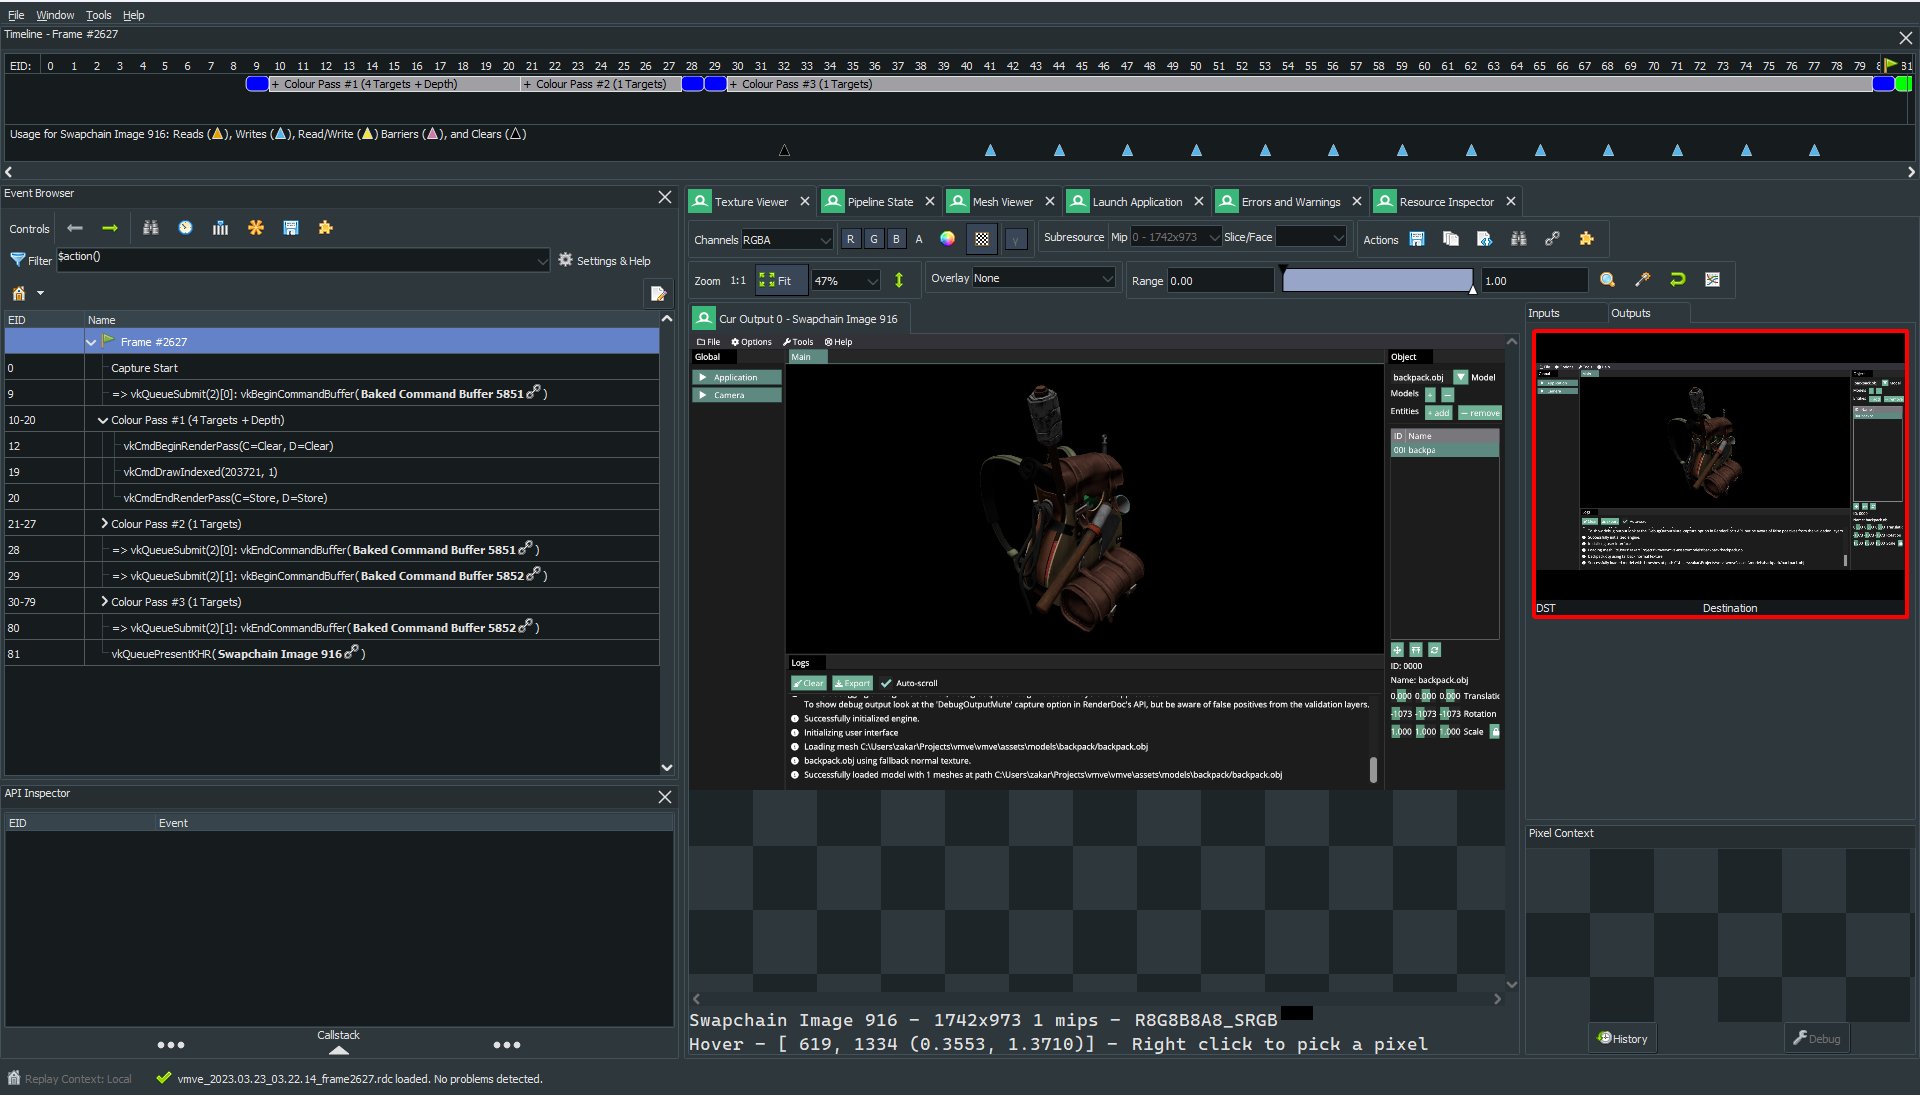
\includegraphics[width=\textwidth]{images/renderdoc.png}
  \caption{RenderDoc}
  \label{fig:renderdoc}
\end{figure}

\subsubsection{AMD Radeon GPU Profiler}
Similarly, AMD has their own \gls{gpu} profiling tool called ``AMD Radeon GPU
Profiler'' \cite{rgp}. As mentioned above, the hardware used for development
made use of a AMD \gls{gpu}. Therefore, in order to access insightful
performance metrics on a per-frame basis this tool was required and can be 
seen in action in figure \ref{fig:amd_profiler}.

\begin{figure}[h!]
  \centering
  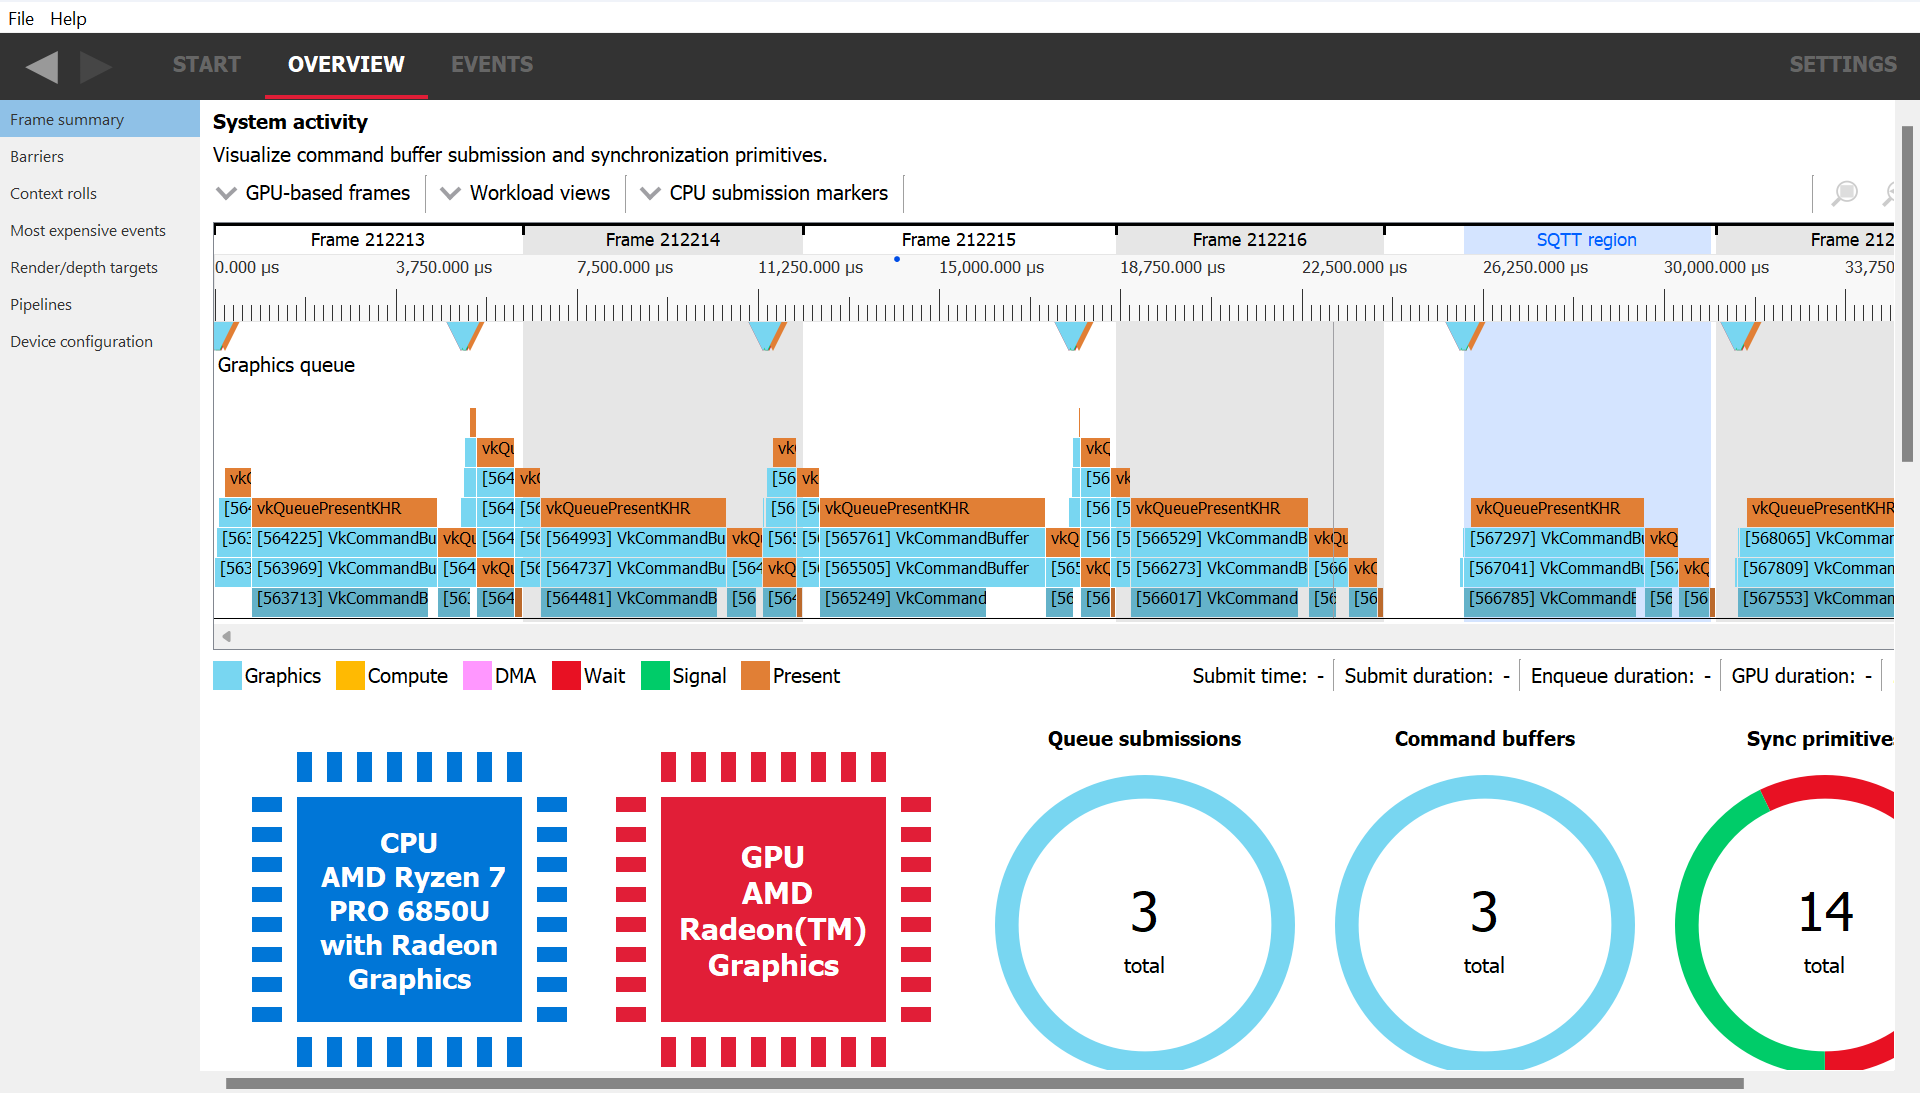
\includegraphics[width=\textwidth]{images/amd_profiler.png}
  \caption{AMD Radeon GPU Profiler}
  \label{fig:amd_profiler}
\end{figure}


\subsection{Programming Language}
Due to the nature of application, there were several requirements that had to be
met such as a high performing programming language as well as low-level memory
access in order to specifically manage how memory is handled within the
application.

The language chosen for this project was C++ 23.  There were two main reasons
as to why this specific programming language was chosen. Firstly, it's the language
that I have the most experience with which would significantly help during the 
implementation stages of the project. The second reason is the \gls{stl} STL (Standard
Template Library) was one of the key reasons as to why I ended up
choosing this specific programming language. It provides many prebuilt
data structures and containers including ``std::vector'', ``std::string'',
``std::find'' etc. that are really helpfully in managing the data in the application.
Furthermore, it saves time as I would not have to implement my own solution
in the limited time-frame that I have.

Other language features that solidified by choice include, function overloading,
templates, compile-time expressions, direct memory access and generally faster
performance compared to higher level languages such as Python and Javascript.

\subsection{Rendering API} \label{rendering_api}
One of the core aspects of \gls{vmve} is making use of the underlying hardware and
more specifically the GPU (Graphics Processing Unit) which will be primarily
used for rendering. Taking advantage of the GPUs hardware capabilities requires
low-level access to the hardware and is not as straightforward as one would
hope. To understand why, we must first understand how Graphics Processing Units
function.

There are different types of GPUs such as dedicated or onboard, different
architectures including AMDs RDNA \cite{RDNA} or NVIDIAs ADA \cite{ADA} as well
as various capabilities that differ between hardware vendors. An application
attempting to target GPUs would need to take this all into consideration
including having access to the GPU drivers (Low-level software that allows a
specific piece of hardware to function). Often times, drivers are considered
trade secrets that companies do not want freely available. Given the complexity
and variations of modern GPUs this is simply not feasible.

Companies from across the different industries solved this issue by creating
an open, non-profit consortium in early 2000s called The Khronos Group. This
organization develops, publishes and maintains standards for different areas
but most notably for 3D Graphics and Computation. Companies follow these 
standards when developing software allowing for interoperability across
hardware. As of 2023, The Khronos Group actively maintains 16 different
standards. Out of all those standards, there are two which are the most
suitable for VMVE, OpenGL and \gls{vulkan}.

OpenGL and \gls{vulkan} are two types of rendering APIs that designed based on
The Khronos Group specifications. When attempting to provide graphics support
for a particular \gls{gpu}, hardware vendors follow the OpenGL and/or \gls{vulkan}
specifications when implementing their drivers. For applications, a
\acrfull{api} is provided allowing for direct control of the \gls{gpu}.

\gls{vmve} could support both OpenGL and \gls{vulkan} however, due to the vasts
amount of work required to accomplish this as well as the projects time
constraints this is simply not feasible. Instead, both need to be evaluated with
the aim of choosing one.



// CONTINUE FROM HERE

adhere to the OpenGL specification

- Why am I going to be using Vulkan instead of OpenGL?
-   Finer control of rendering pipeline
-   Aiming to learn and have a deeper understanding of low-level GPU architecture
-   Using Vulkan means that we avoid OpenGLs state machine architecture.
    can introduce bugs
-   Reduced driver overhead
-   Allows for finer control of multithreading
-   Better performance potential
-   Error checking can be disabled when shipping application.



\subsection{Libraries}

\subsubsection{User Interface}
Users will need a way of interacting with \gls{vmve} and the 3D environment.
This will be achieved through the use of a user interface in which the user can
directly manipulate the application. As mentioned earlier, \gls{vmve} is a
application that uses the \gls{gpu} for rendering and therefore, the UI will
have to interact with the \gls{gpu}. To reduce the development time of this
particular aspect of the application, the decision was made to make use of a
preexisting library.

The library of choice was Dear ImGui \cite{imgui}. This is an immediate-mode
user interface library that provides an \gls{api} in order render UI elements. 

\subsubsection{Encryption} \label{custom_file_format} VMVE will include its own
model file format. This is a special format that will be encrypted as standard.
Implementing encryption is a very complex area that can be considered an entire
project on its down. Instead, the project will make use of a well known
encryption library known as Crypto++ \cite{cryptopp}. This is a C++ library that
provides various algorithms including AES, Diffie-Helm, 

\section{Design}

Having discussed the different technologies being used in VMVE, they must now be
evaluated and incorporated into the design of VMVE and its various subsystems.

\subsection{Project Name}
VMVE stands for ``Vulkan Model Viewer and Exporter''. The name is mainly split
into two halves. The first is ``Vulkan'' and the other is ``Model Viewer and
Exporter''. Fundamentally, the application revolves around the idea of being able
to view/manipulate 3D digital assets and export them into a custom file format
as mentioned in section \ref{custom_file_format}.

\subsection{Branding}

There are two versions of the VMVE logo that were designed and are intended to
be used in different situations. The first is the complete large logo as seen
below in figure {}

\begin{figure}[h!]
  \centering
  
\includegraphics{images/project_logo.png}
  \caption{VMVE Large Logo}
  \label{fig:project_logo_large}
\end{figure}

The second version is designed to be minimal and therefore, only consists of the
icons itself.

\begin{figure}[h!]
  \centering
  
\includegraphics{images/project_icon.png}
  \caption{VMVE Small Logo}
  \label{fig:project_logo_small}
\end{figure}


\subsection{VCS Architecture}

As the only developer for this final year project, the design and architecture
will remain as simple as possible while still providing the core requirements.
Figure \ref{fig:brancharch} shows the proposed version control architecture and
includes to branches named ``main'' and ``develop''. Develop will be the primary
branch used throughout the implementation stages. 

Main will be used as a stable branch that is only updated for each official release.
This would occur for each project milestone such that for ``Sprint 1'' a pull request
will be made from develop to main and this will be tagged as v0.0.1 and likewise 
``Sprint 2'' will be tagged as v0.0.2.

\begin{figure}[h!]
  \centering
  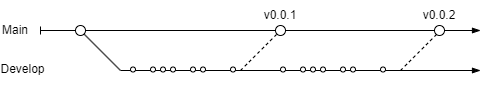
\includegraphics[width=\textwidth]{images/current_branch_design.png}
  \caption{Git branch design}
  \label{fig:brancharch}
\end{figure}

\subsection{Programming Conventions}
From the beginning, the projects source code and overall architecture was to
adhere to the C++ Core Guidelines \cite{cpp-guidelines} to ensure that the
project follows best practices.

Significant amount of consideration was spent planning out a suitable project
wide programming style. In regards to naming, section
\href{http://isocpp.github.io/CppCoreGuidelines/CppCoreGuidelines#nl10-prefer-underscore_style-names}{NL.10}
of the core guidelines recommends using ``underscore\_style'' naming as it follows
the standard libraries naming convention. Since the VMVE project has no existing
code base and therefore, no existing convention to follow, the project will
make use of the underscore style for types, functions and variables. 

Additionally, section
\href{https://isocpp.github.io/CppCoreGuidelines/CppCoreGuidelines#nl17-use-kr-derived-layout}{NL.17}
states that the use of the ``K\&R''  indentation style \cite{indentation} should
be used as it preserves vertical space whilst maintaining readability. In other
words, reduces vertical line height for code blocks such as ``if, else, while,
for'' allowing for more lines of code to be visible at any given point whilst
allowing for a more distinct separation for structures and functions.

The combination of these two specific conventions in regards to source
code style can be seen in figure \ref{fig:convention}.
\begin{figure}[h!]
  \begin{verbatim}
    struct foo
    {
        int a;
    };

    void bar(int a)
    {
        if (a) {
            printf("This is a example.\n");
        } else {
            printf("This is another example.\n");
        }
    }
  \end{verbatim}
  \caption{Example code structure}
  \label{fig:convention}
\end{figure}



\subsection{Project Architecture}

\begin{figure}[h!]
  \centering
  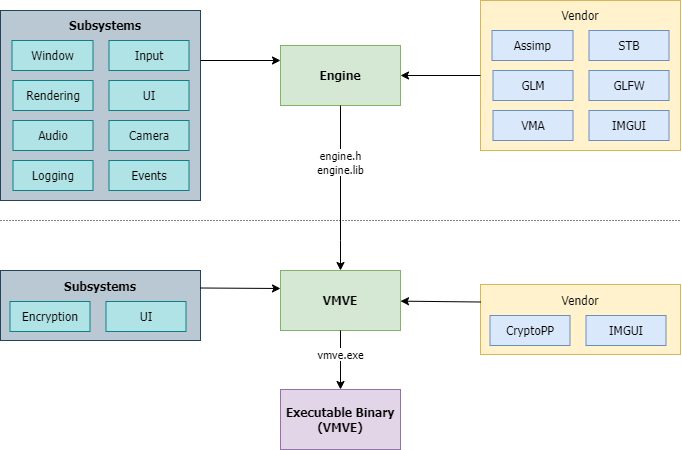
\includegraphics[width=\textwidth]{images/project_architecture.png}
  \caption{Project Architecture}
  \label{fig:projarch}
\end{figure}
VMVE will be a combination of two projects. The ``Engine'' project
also known as the core of VMVE will contain the fundamental
implementation details. This includes the window, renderer, ui and
other subsystems. This project will be distributed as a library
file (.lib) that other projects can import for specific use cases.

The ``VMVE'' project will include the ``Engine'' project by importing
the .lib file.

A high-level overview of the project architecture can be seen in
figure \ref{fig:projarch}.

There is another key reason as to why, I will isolate the core of VMVE
into its own project instead of combining it into one program. The
reason being is have the core be a library that can be used in not
just VMVE but also other projects in the future.








- Reason for choosing 64bit program.
    goes beyond 4GB address space limit in 32bit programs.
    supports modern hardware

- Functional over object oriented
-   POD (Plain old data types)
-   Less boilerplate code (getters and setters)
-   Easier access to member variables

- Editor UI design and the reason for it for this particular application?
-   UI allows for interaction with underlying system during runtime.
-   Viewport style editor meaning that all controls can be positioned
    around the viewport and the main rendering occurs at the center of
    the screen.
- VMVE file format
-    Header
-    Data
- Encryption
- AES (128, 256 bits for key length)



\subsection{Renderer Architecture}

As mentioned in section \ref{rendering_api}. Vulkan will be the rendering API of choice
for VMVE. The API is extremely verbose giving the programmer the flexibility to
control every aspect of the GPU. When interacting with Vulkan throughout the engine
a certain degree of encapsulation is necessary to reduce the amount of effort required to 
implement functionality as a result of Vulkans' verbose API.

To achieve this, the renderer must be properly designed so that flexibility is not lost
whilst still simplifying the API. Figure \ref{fig:rendererarch} shows the proposed renderer
architecture which makes distinctive boundaries and encapsulates key systems.

\begin{figure}[ht]
  \centering
  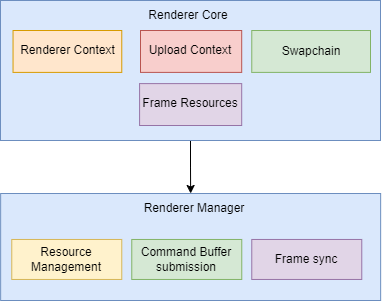
\includegraphics[width=\textwidth]{images/renderer_architecture.png}
  \caption{Renderer Architecture}
  \label{fig:rendererarch}
\end{figure}

\subsection{User Interface}
Designing the user interface was the next step as part of the design stage of
the project. Figure \ref{fig:ui_design} shows the initial user interface
wireframe that includes four main elements titled ``Global Controls'', ``Logs'',
``Model Controls'' and ``Main Viewport''. Each of these UI elements are located
in their respective windows which are designed in such a way that common controls are group
together and located appropriately if not within the same panel.

\begin{figure}[ht]
  \centering
  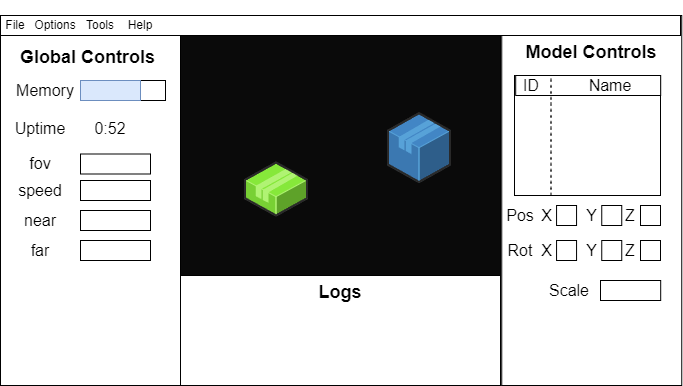
\includegraphics[width=\textwidth]{images/ui_design.png}
  \caption{UI Design}
  \label{fig:ui_design}
\end{figure}

\subsubsection{Main Viewport}
The main viewport is located in the center of the window and is the main feature
of the user interface. The viewport displays the virtual environment and 

\subsubsection{Global Controls}

\subsubsection{Model Controls}

For each model loaded into the application and currently highlighted, is shown
model specific information within the model controls panel. This panel will include various 


\subsubsection{Logs}
The logs panel is designed to contain all internal messages that the application
prints out. These messages will then be displayed within the logs panel. Each
log message will be categorized as either log, warning or error. Depending on
which log type the message is, it will be shown in a different color such as
white, orange or red respectively.

This is designed so that the user will have a clear understanding of the internal state
of the application.

\subsection{Custom file format and encryption}

\subsubsection{File format}
VMVE will include its own file format that allows for model data to be encrypted for security purposes.
Figure \ref{fig:vmve_file_structure} shows the proposed internal structure of the custom file format.
It includes a 48 byte header that will consist of a version and the method used for encryption.
The purpose of the version is to check for compatibility between different VMVE versions. In addition to this,
this can used to convert older versions of a VMVE to newer versions.

The second item in the VMVE header is the encryption mode. This allows for the VMVE to know which algorithm
must be used to decrypt the data.

-- TODO: Update picture to use a smaller header size by using a packed uint32\_t for the version

\begin{figure}[ht]
  \centering
  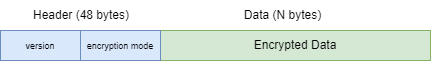
\includegraphics[width=\textwidth]{images/vmve_file_structure.png}
  \caption{VMVE File internal structure}
  \label{fig:vmve_file_structure}
\end{figure}


\subsubsection{Encryption and Decryption}
-- encrypting --
-- loading model
-- encrypting model
-- export model


-- decrypting --
-- load model 
-- check version
-- check encryption mode
-- attempt to decrypt
-- load model into VMVE

\section{Implementation}
This section of the report presents the technical implementation details of
VMVE. This section is presented in order of initialization i.e starting at
the core of the application and discussing each subsequent system.

\begin{figure}[h!]
  \centering
  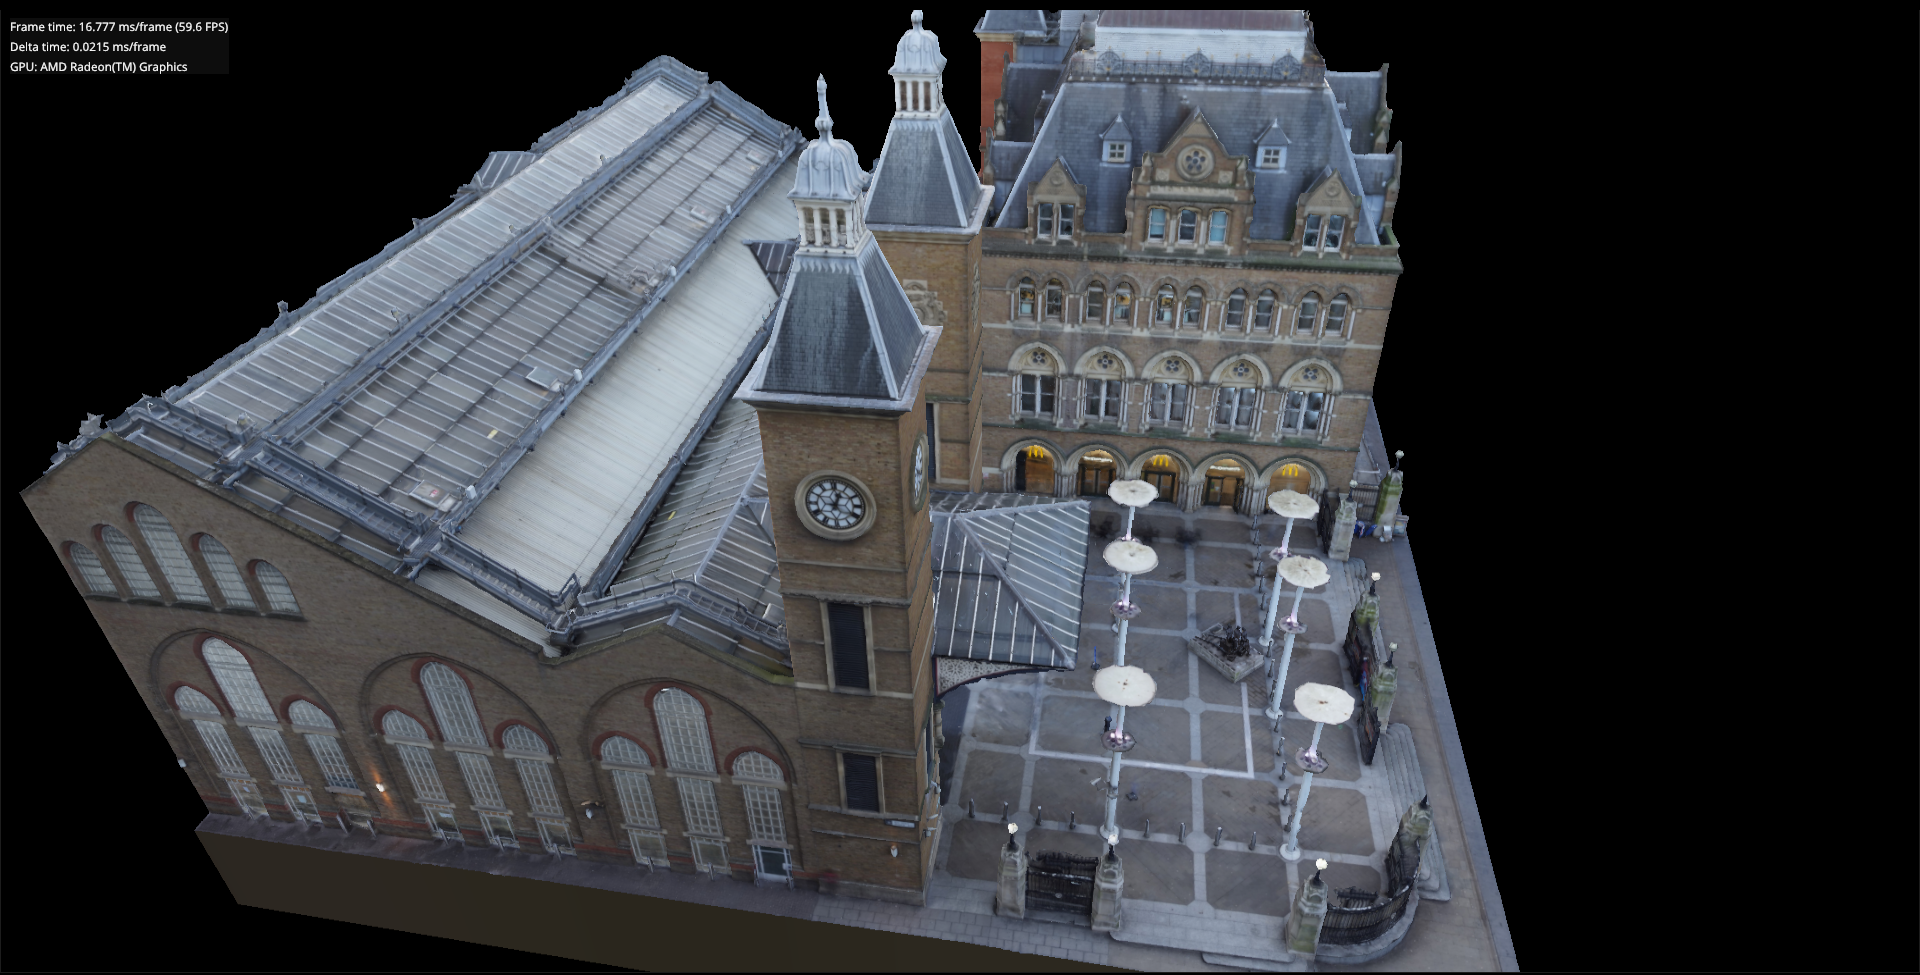
\includegraphics[width=\textwidth]{images/rendering.png}
  \caption{Liverpool Street Station renderer model}
  \label{fig:renderer}
\end{figure}


\subsection{Overview}
Figure \ref{fig:overview_pseudo_code} shows the general overview of the application and the various 
stages that occur during initialization, runtime and shutting down.


\begin{figure}[ht]
\centering
\begin{lstlisting}[language=C++]

int main()
{
  // begin application initialization
  create_window(width, height, name);
  create_renderer();
  create_audio();
  create_ui();

  // set default configuration options
  create_camera();
  
  // begin application rendering
  while (running)
  {
    update_renderer();

    render_geometry();
    render_ui();

    update_window();
  }

  // shutdown application
  destroy_ui();
  destroy_audio();
  destroy_renderer();
  destroy_window();

  return 0;
}
\end{lstlisting}
\caption{Implementation overview pseudo code}
\label{fig:overview_pseudo_code}
\end{figure}

  

\subsection{Window System}
The first system within VMVE that gets initialized is the window. This system is
responsible for creating a desktop window based on a series of configuration
options specified at the start of the application. These options include the
window width, height and name. Internally, VMVE uses the lightweight GLFW
library to handle window creation. The purpose of this library is to provide an
API which is cross platform and allows applications to easily create windows on
different operating systems. 

Under the hood, on Windows, GLFW uses the Win32 API provided by Microsoft.

In addition to the window creation, various function callbacks are created
which allow VMVE to handle specific events such as window resizing, input,
cursor position etc.

\subsection{Rendering System}

The implementation of the rendering system was one of the key areas
I worked on throughout the course of the project.

The 

This is one of the key systems of the engine and subsequently VMVE.
 Linking against actual driver function calls instead of linking to
 the common Vulkan loader.  \cite{volk}

- Renderer context Combine Vulkan resource allocating objects into
-   single object for increased clarity 
    Frames in flight 
    Double and

64 bit world positions 
Shader resources SPV binary format 
    Pipelines
-   Pipeline cache 
Pipeline derivitive 
Delta Time

- Matrix projection transformation (model to projection space)


\subsubsection{Renderer Context}
\begin{lstlisting}[language=C++]

struct vk_context
{
  VkInstance         // Initializes Vulkan library
  VkPhysicalDevice   // Handle to physical hardware
  VkDevice           // Logical handle to physical hardware
  VkQueue            // Graphics queue
  VkQueue            // Presentation queue
  VmaAllocator       // VMA memory allocator
};


\end{lstlisting}

\subsubsection{Presenation}

- Double, Triple Buffering
- VSync

\subsubsection{Framebuffers}

\subsubsection{Texture sampling}

\subsubsection{Deferred Rendering Pipeline}

-- Explain what forward rendering is, what deferred rendering is and how it is better

At its core, the renderer uses a deferred rendering technique which separates geometry rendering and
lighting into different stages. 

The key benefit of deferred rendering is increased performance 

\begin{figure}[h!]
  \centering
  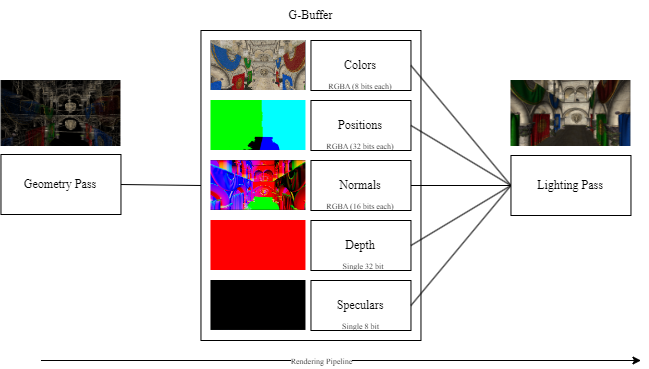
\includegraphics[width=\textwidth]{images/g_buffer.png}
  \caption{G-Buffer Pipeline}
  \label{fig:g_buffer}
\end{figure}

\subsubsection{Dynamic Uniform Buffers}
-- Per frame uniform buffers consist of data packaged into a single buffer for 
better performance and are accessed by using a frame index counter
-- reduces the need to manage unique buffers, fewer state changes (binding).

-   Triple Buffering Buffers Single large buffer rather than multiple buffers for each frame

\begin{figure}[h!]
  \centering
  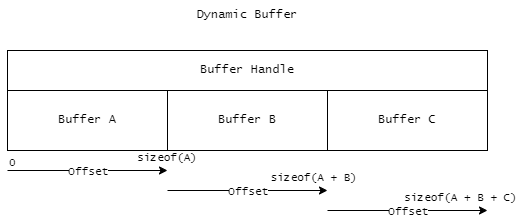
\includegraphics[width=\textwidth]{images/dynamic_buffer.png}
  \caption{Dynamic Uniform Buffer}
  \label{fig:dynamic_uniform_buffer}
\end{figure}


\subsubsection{Frame synchronization}
-- How frames are handles

VkSemaphore
VkFence

\begin{figure}[h!]
  \centering
  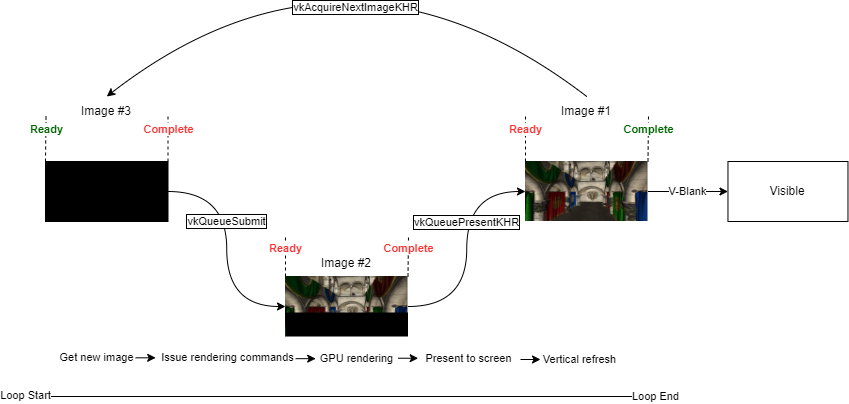
\includegraphics[width=\textwidth]{images/frame_sync.png}
  \caption{Frame Synchronization}
  \label{fig:frame_sync}
\end{figure}



\subsubsection{Model}
In the context of the rendering system, a ``model'' is a structure that represents
a 3D geometry object. This could be as simple as a cube or as complex as an
entire scene.

The data structure contains several key pieces of information such as geometry data
and textures. 

Often times complex models are not singular pieces of geometry. Instead, artists
combine multiple smaller objects together to form the final model. These smaller
parts are known as ``Meshes'' within the application.

Figure \ref{fig:model} shows the internal structure of a example model which has been
loaded into VMVE.
\begin{figure}[h!]
  \centering
  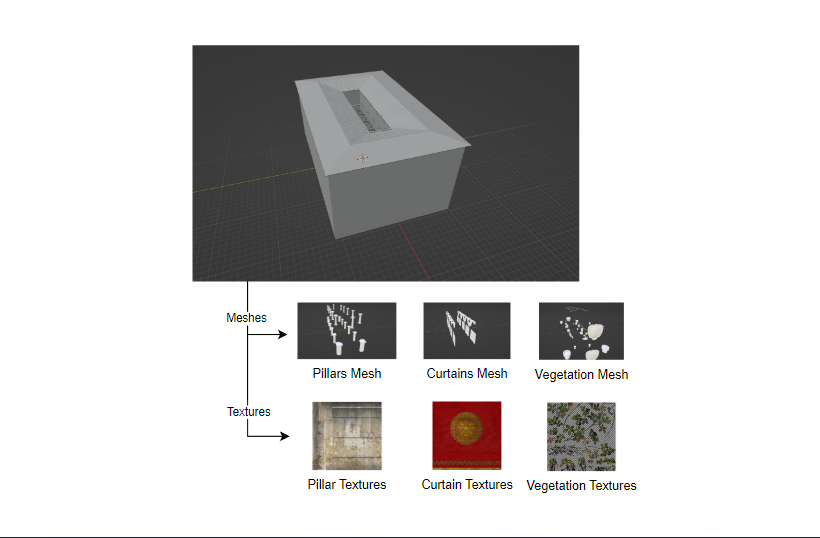
\includegraphics[width=\textwidth]{images/model.png}
  \caption{Model Structure}
  \label{fig:model}
\end{figure}

\subsubsection{Entity}
-- Contains information about what model is being used and a transformation


\subsubsection{Camera}
3D geometry data must be transformed through a series of mathematical
calculations that will take vertex points from a 3D ``world'' and them convert
them onto a 2D image for it to then be displayed on a monitor. This
transformation is known as perspective projection \cite{3d_projection} and is
accomplished by computing several intermediate coordinate spaces as seen in
figure \ref{fig:mvp_projection}.

\begin{figure}[h!]
  \centering
  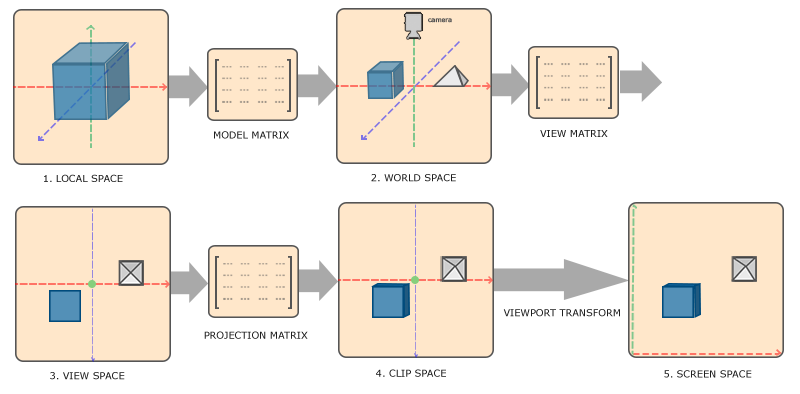
\includegraphics[width=\textwidth]{images/mvp.png}
  \caption{MVP Transformation \cite{coordinate_systems}}
  \label{fig:mvp_transformation} 
\end{figure}

Geometric data is first created within a local coordinate space. This ``space''
is positions relative to the object. In other words, the model data imported by
VMVE will be in this local coordinate system often created by a 3D modelling
program such as Blender or 3DSMax.

The next step is to convert these local coordinates to ``world'' space. This is
the actual virtual environment that an object will live in. The transformation
to this space is done by constructing a 4x4 matrix and performing a combination
of translation, rotation and scaling. A pseudo code example can be seen in
\ref{fig:local_to_world}.

\begin{figure}[ht]
  \centering
  \begin{lstlisting}[language=C++]
    mat4 model = mat4(1.0f);       // Identity matrix
    model = translate(position);   // Move object
    model = rotate(radians, axis); // Rotate object
    model = scale(scale);          // Scale object
  \end{lstlisting}
  \caption{Model matrix construction}
  \label{fig:local_to_world}
\end{figure}
  

The next step is transforming the world space positions to view space or also
known as camera space. This is important as how the virtual scene is displayed
depends on the properties of the camera. In the context of graphics rendering
the concept of a ``camera'' does not exist and is only really an illusion. In
reality, all points/vertex positions in the world space are transformed relative
to the ``camera''. For example, if the cameras position along the z axis
increases i.e. we move forward then all objects in the world will be moved
towards us. A nice visualization of this is shown in figure
\ref{fig:camera_projection} curtesy of a blog post by \href{Jordan
Santell}{https://jsantell.com/model-view-projection/}.

\begin{figure}[h!]
  \centering
  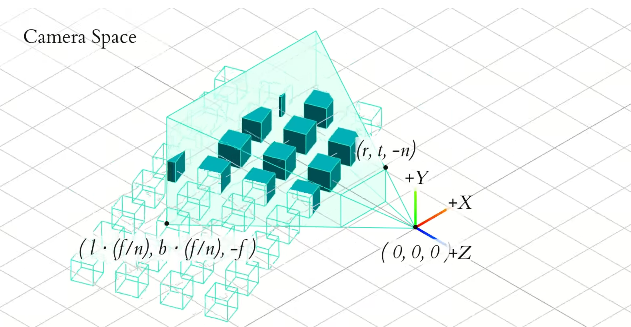
\includegraphics[width=\textwidth]{images/camera_space.png}
  \caption{Camera/view projection \cite{camera_projection}}
  \label{fig:camera_projection} 
\end{figure}

\gls{vmve} makes use of a quaternion to perform the view projection. This is an
alternative to euler angles and has several benefits including, preventing gimbal
lock and easier interpolation between orientations.
\begin{figure}[ht]
  \centering
  \begin{lstlisting}[language=C++]
    mat4 view = lookAt(camera_position, view_direction, camera_up);
  \end{lstlisting}
  \caption{View matrix construction}
  \label{fig:world_to_view}
\end{figure}


The final step in calculating the MVP matrix is the projection which converts
points from local space to clip space. This involves projecting the points to
either a perspective or orthographic projection.
\begin{figure}[ht]
  \centering
  \begin{lstlisting}[language=C++]
    mat4 proj = perspective(fovy, aspect, near, far);
  \end{lstlisting}
  \caption{Projection matrix construction}
  \label{fig:local_to_projection}
\end{figure}

With the fully constructed mvp matrix, this can now be multiplied with each
vertex position and it will display onto the screen as expected.
\begin{figure}[h!]
  \centering  
  \begin{equation}
    Output = MVP \times Vertex
  \end{equation}
  \caption{MVP projection}
  \label{fig:mvp_projection}
\end{figure}

A more detailed code example can be seen in figure
\ref{fig:local_to_world_appendix} in the appendix.

\subsubsection{Lighting}

The lighting model that is implemented in Blinn-Phong which derives
from the original Phong model developed by By Bui Tuong Phong in a
paper published in 1975.  Purpose of lighting model is to calculate
approximations of lighting based on the real world.  \cite{blinn}

Ambient is a constant value that is used instead of global illumination
as it requires more computational resources and more complex algorithms.

\newcommand{\intensity}{\operatorname{I}}
\newcommand{\lightdir}{\operatorname{L}}
\newcommand{\normal}{\operatorname{N}}
\newcommand{\diffuse}{\operatorname{D}}
\newcommand{\glslcolor}{\operatorname{C}}
\newcommand{\glslmax}{\operatorname{max}}

\begin{equation}
	A = G + P
\end{equation}

The next step is implementing diffuse lighting. This takes into account
the light direction $\lightdir$ and the normal $\normal$ for a surface at a particular
pixel. The formula below calculates the intensity at which light reflects off the
of an object based on the angle the surface is against a light source. 

The dot product of the light direction and surface normal returns a value between
the ranges of -1 to 1 depending on how parallel the directions are. If this value
is less than 0 then it's clamped as a result of the max function which returns the largest value for the given two parameters.
\begin{gather}
	\intensity = \glslmax(\vec{\lightdir} \cdot \vec{\normal}, 0) \\
\end{gather}

Having calculated the intensity value we can now simply multiply it with the objects
surface colour.
\begin{equation}
	\diffuse = \intensity \times \glslcolor
\end{equation}

Figure \ref{fig:diffuse} demonstrates the use of diffuse lighting which shows how each
surface of the cube is lit differently based on its angle to the directional light 
source. 
\begin{figure}[h!]
  \centering
  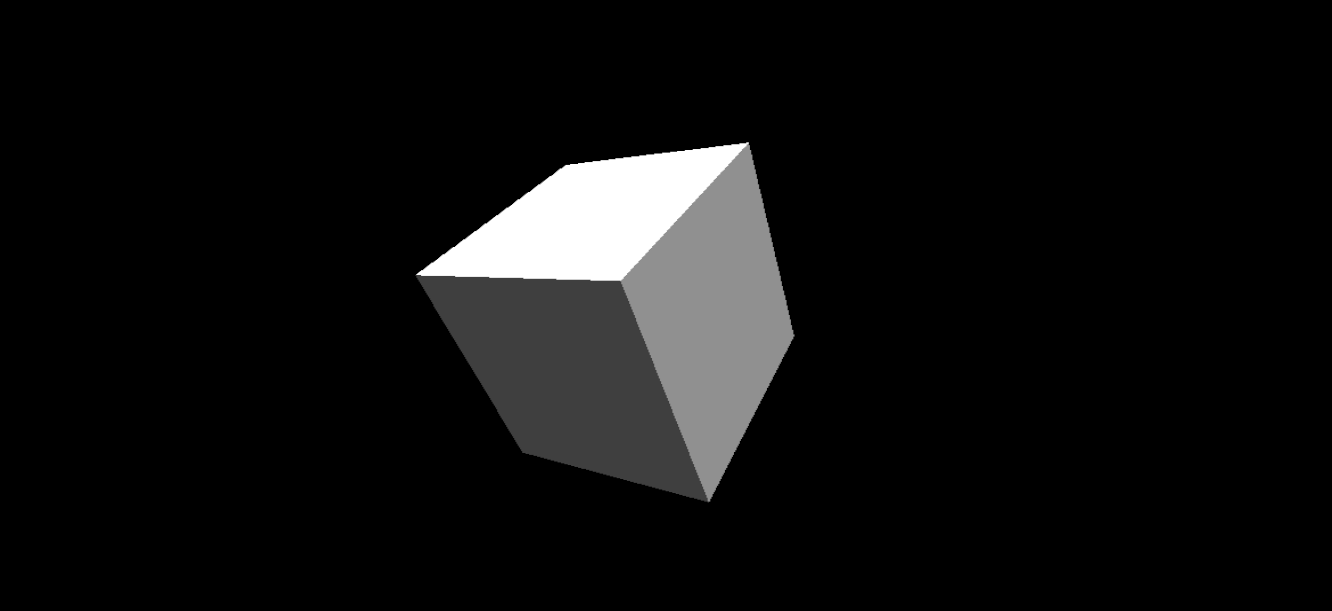
\includegraphics[width=\textwidth]{images/diffuse_lighting.png}
  \caption{Diffuse Lighting}
  \label{fig:diffuse}
\end{figure}


The final step in the Blinn-Phong lighting model is specular highlighting. This effect
adds...


\subsection{User Interface}
The implementation of the user interface was the next major element. This is
the frontend and how the users will be able to interact with the application.

\begin{figure}[h!]
  \centering
  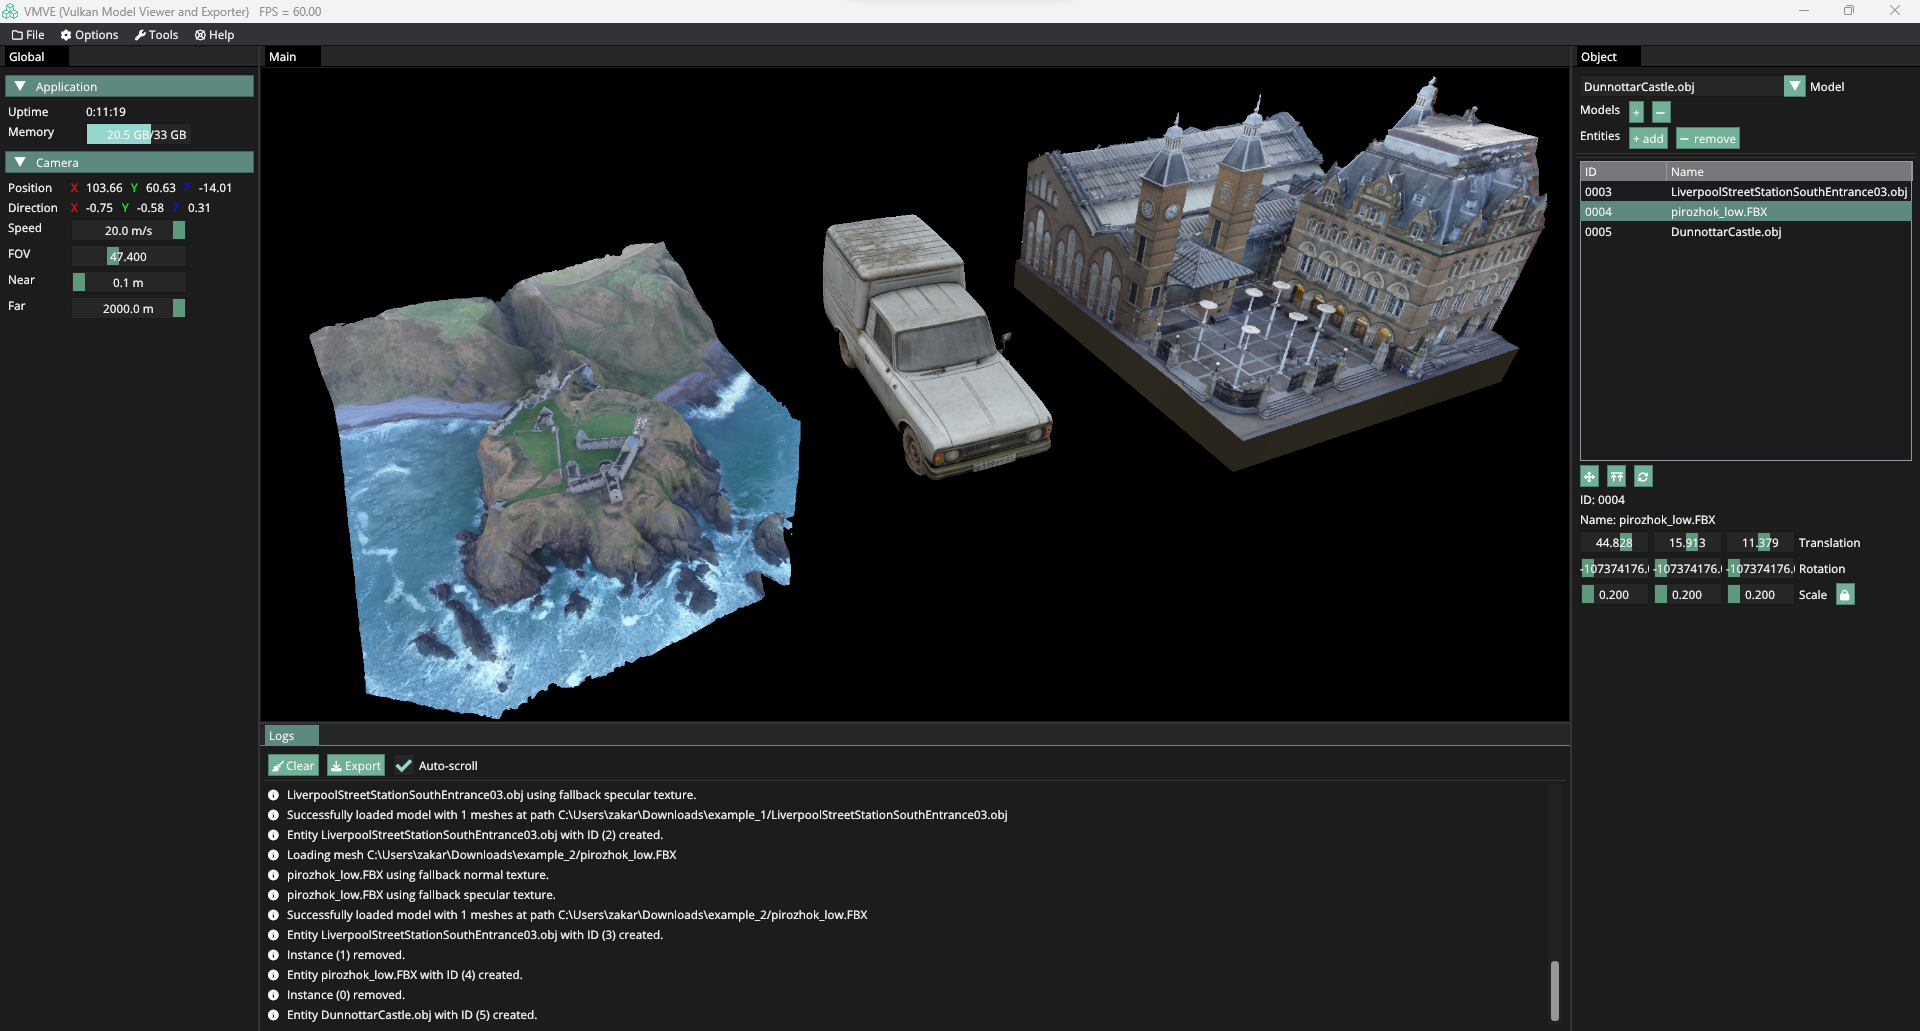
\includegraphics[width=\textwidth]{images/ui_implementation.png}
  \caption{UI implementation}
  \label{fig:user_interface}
\end{figure}


\subsubsection{Fonts and Icons}
The font used for the user interface is Open Sans which provides a simple and
easy to read font.

\gls{vmve} also uses icons throughout the user interface and is an important
aspect in conveying key information such as the task being performed or for
additional information. The icon font used is provided by Font Awesome
\cite{font-awesome}.

Typically, data for fonts and icons are stored in a font file which end using
extensions such as ``.ttf'' or ``.otf''. However, one of \glspl{vmve} goals is
to be distributed as a single executable file. Therefore, we cannot depend on
external font files. Instead, data for fonts and icons are stored directly in
the application in a continuous array of bytes and are encoded in base85. An
small example of what this looks like can be seen in figure
\ref{fig:base85_font}. The full version of this is over 3000 lines long due to
the vast of amount of data stored within the font.

\begin{figure}[h!]
  \centering
  \begin{lstlisting}[language=C++]
    // 206 out of 201650 characters are shown

    const char open_sans_regular[201650 + 1] =
    "7])#######2Pc7('/###I),##d-LhLjKI##4%1S:`*]n8)K.v5*8_c)iZ;99=$$$$c(m]4pKdp/(RdL<snZo'oI,hLNDnx4Uu/>8Q7oo^eFb3hB4JYc'Tx-3l_wgd2Tf._r+&sAqV,-G"":F8LD=5,n]A&aA+<gXG-<iobW&>$>QJ8Z.W$jg0Fv-o^(^JJnf4T"
  \end{lstlisting}
  \caption{Base85 encoded font}
  \label{fig:base85_font}
\end{figure}

\subsubsection{Menu Bar}

\begin{figure}[h!]
  \centering
  
\includegraphics[width=\textwidth]{images/menu_bar.png}
  \caption{Menu Bar}
  \label{fig:menu_bar}
\end{figure}


\subsubsection{Load Model Window}
\begin{figure}[h!]
  \centering
  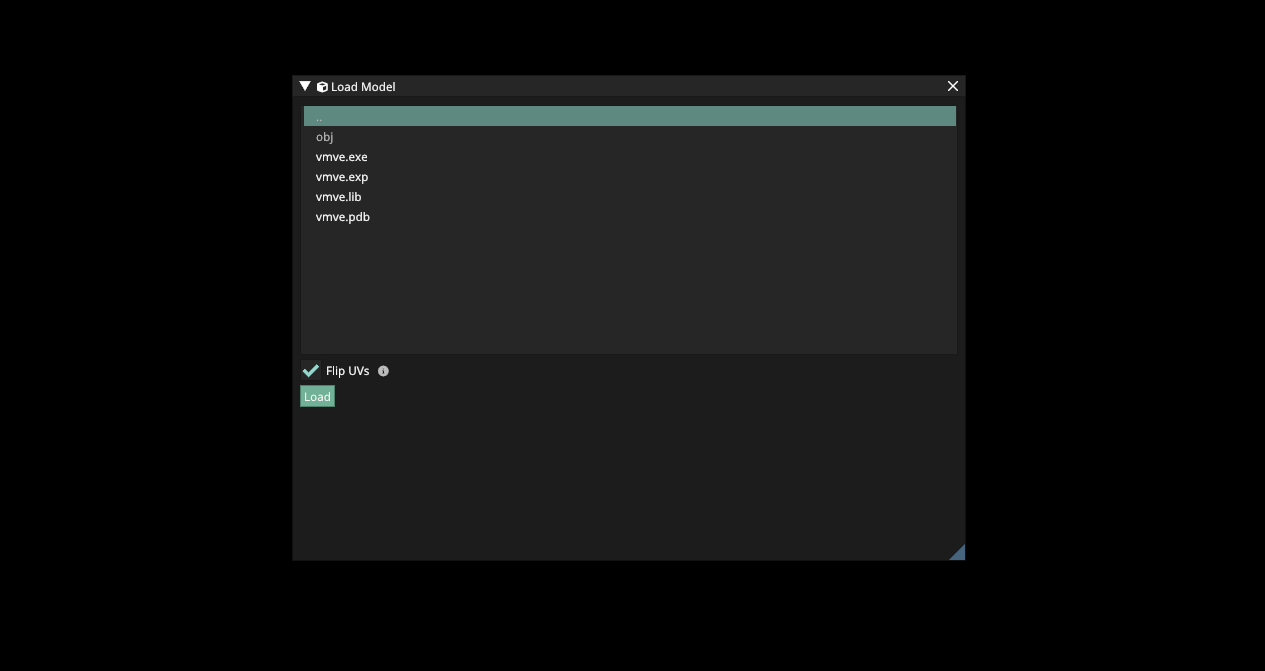
\includegraphics[width=\textwidth]{images/load_model_window.png}
  \caption{Load Model Window}
  \label{fig:load_model_window}
\end{figure}


\subsubsection{Export Model Window}
\begin{figure}[h!]
  \centering
  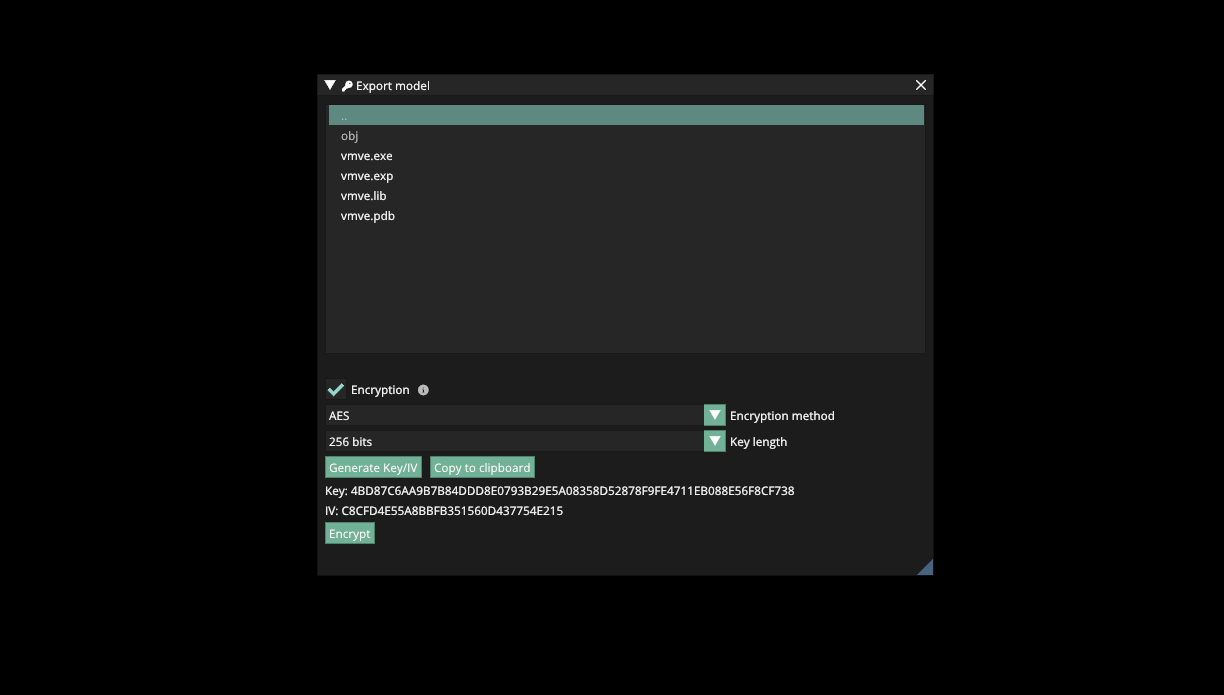
\includegraphics[width=\textwidth]{images/encryption_system.png}
  \caption{Export Model Window}
  \label{fig:encryption_window}
\end{figure}

\subsubsection{Settings Window}

\begin{figure}[h!]
  \centering
  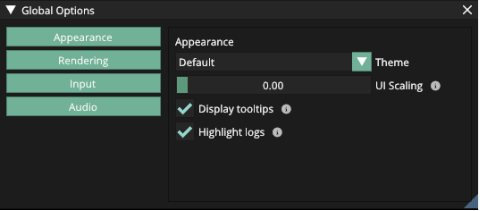
\includegraphics[width=\textwidth]{images/settings_window.png}
  \caption{Settings Window}
  \label{fig:settings_window}
\end{figure}

\subsubsection{Object gizmo}
An additional feature that is part of the user interface is the gizmo. This is a
visualization of one of three operations is the main method of interaction that
a user has with an object and is used to specify the exact location and
orientation within the virtual environment. The operations are translation
(moving), rotation and scaling and can be seen in figure \ref{fig:gizmo}
respectively.
\begin{figure}[h!]
  \centering
  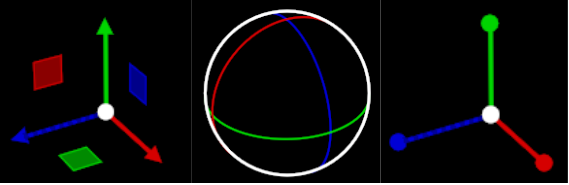
\includegraphics[width=\textwidth]{images/gizmo.png}
  \caption{Gizmo operations}
  \label{fig:gizmo}
\end{figure}

This functionality is implemented by taking the matrix transformation of an
object and feeding that information to ImGuizmo \cite{imguizmo}. It will then
perform the necessary mathematical calculations to convert from the objects
world space to screen space. In other words, no matter where in the virtual
environment the object is located, it will always be shown relative to the users
screen. A small code snippet can be seen below \ref{fig:imguizmo_code} where
\(M\) represents the model in the \(MVP\) projection.


\begin{figure}[ht]
  \centering
  \begin{lstlisting}[language=C++]
    const auto& operation = static_cast<ImGuizmo::OPERATION>(guizmo_operation);
    const auto& mode = ImGuizmo::MODE::WORLD;
    ImGuizmo::SetDrawlist();
    ImGuizmo::SetRect(x, y, viewport_x, viewport_y);
    ImGuizmo::Manipulate(view, proj, operation, mode, m);
  \end{lstlisting}
  \caption{ImGuizmo world to screen space}
  \label{fig:imguizmo_code}
\end{figure}



\subsection{Logging system}
- Buffer based logging system
- buffer is preallocated ahead of time to increase performance (must be tested)
- once buffer is filled, the oldest log message is deleted

\begin{figure}[h!]
  \centering
  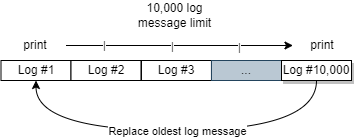
\includegraphics[width=\textwidth]{images/logging.png}
  \caption{Logging FIFO system}
  \label{fig:logging_system}
\end{figure}

\subsection{Encryption System}
-- AES (key and initialization vector)
-- Image of how the system works 
  -- Loads model file, encrypts it and then writes it back out


\subsection{Custom File Format}
-- File Format structure



\subsection{Distribution}
- Release mode (optimized)
- Runs on multiple systems
- Windows only currently

\subsubsection{Versions}
\gls{vmve} follows the major, minor and patch system of versioning and is used
as follows [Major].[Minor].[Patch]. The use of versions is important in
differentiating between VMVE releases. Each new version of the application comes
new features as well as bug fixes that aim to improve the software over time.
Due to the rapid development of new features and functionaility, backwards
compatibility cannot be guaranteed. The current official release of \gls{vmve}
is v0.0.4.

\subsubsection{Website}
Alongside the application, a website was created as a platform for easily
distributing the application. It includes a features section that showcases and
gives users a preview of the application through the use of images and videos.
Futhermore, a download link is provided giving users an easy way of obtaining
the executable without needing to understand the technicalities of GitHub as it
is designed with programmers in mind.

In regards to downloads, there are two types. The first is an active development
version which is regularly updated and acts as a beta release for versions that
have not yet been officially released. The second is current and past VMVE versions
going all the back to the first official release (v0.0.1).

\begin{figure}[h!]
  \centering
  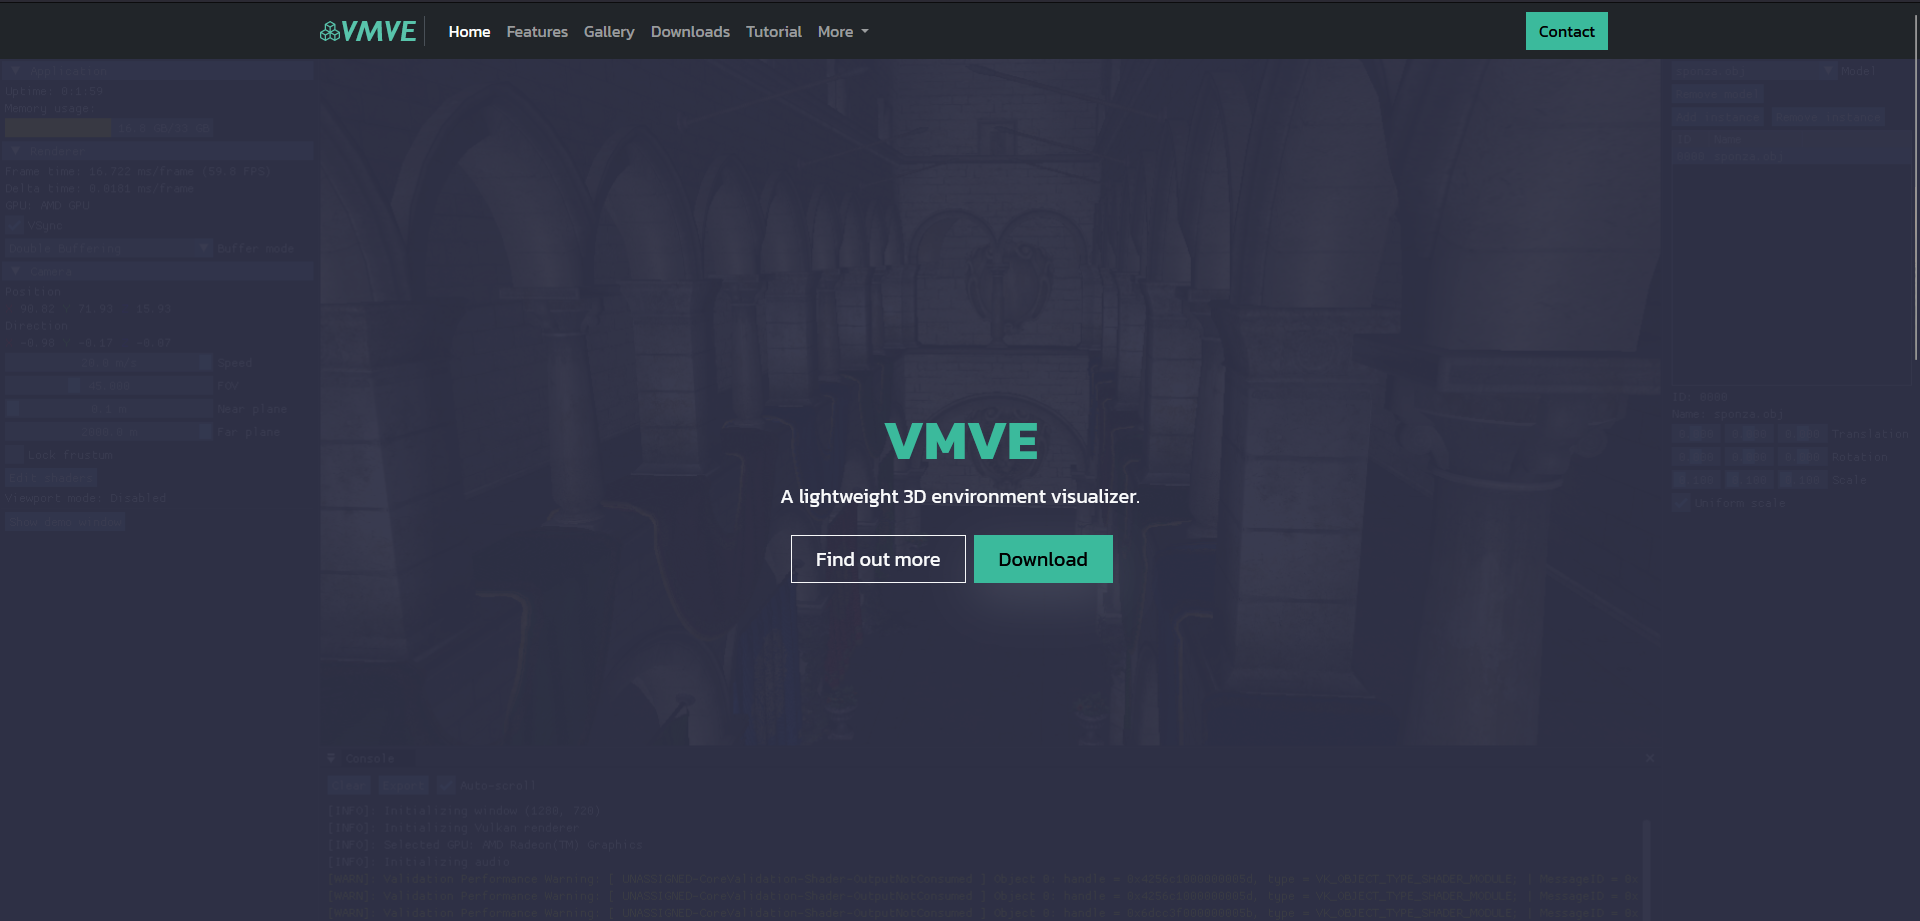
\includegraphics[width=\textwidth]{images/website.png}
  \caption{VMVE website}
  \label{fig:website}
\end{figure}


\subsubsection{Example models}
The VMVE website provides an additional download link to six different example
models. These are provided by third parities (with appropriate credits) and are
corrected to ensure they can be loaded into VMVE without any issues. The purpose
of these example models is to allow users to easily test the application without
needing to search the internet or create their own.


\subsubsection{Documentation}
In addition to a website, a documentation website was also created curticy of
Read the Docs (\href{https://readthedocs.org}{https://readthedocs.org}). The
purpose of this site is to provide additional information about \gls{vmve} and
also provide an in depth tutorial that aims to help users understand and how to
use the application.

This significantly reduces the learning curve and allows new users to quickly
start using \gls{vmve}.

\begin{figure}[h!]
  \centering
  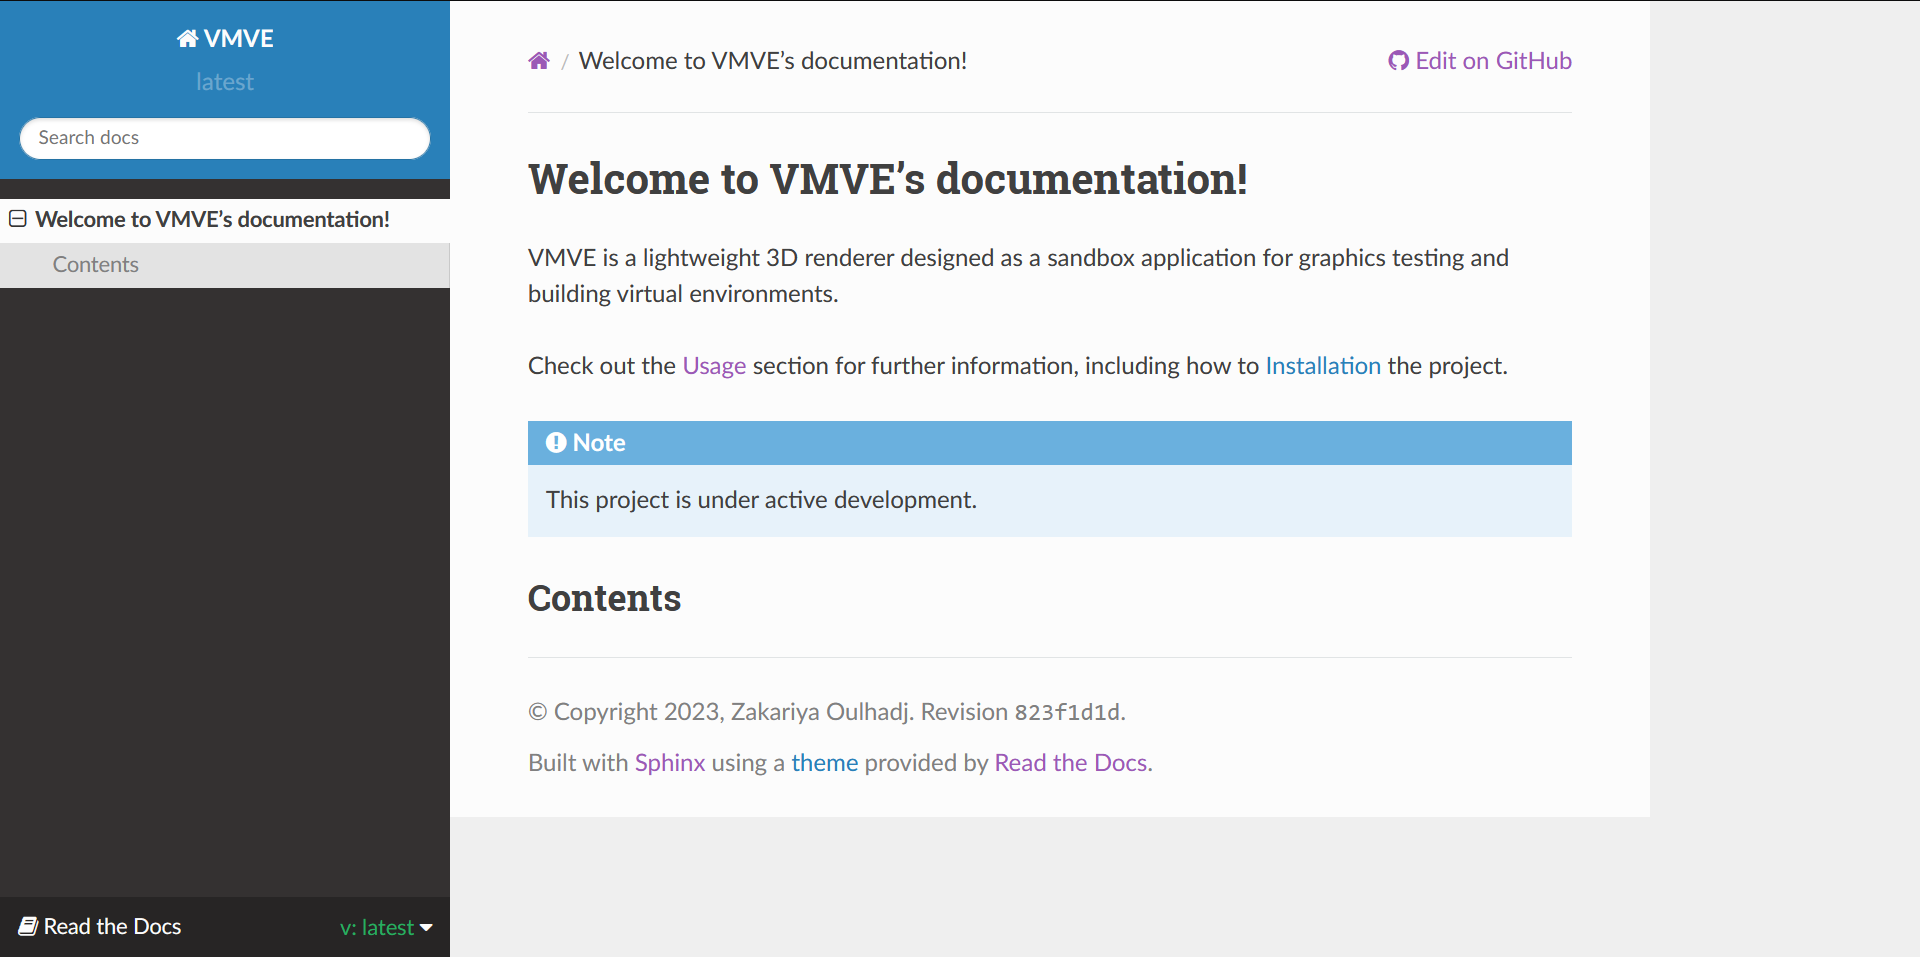
\includegraphics[width=\textwidth]{images/documentation.png}
  \caption{VMVE documentation}
  \label{fig:documentation}
\end{figure}


\section{Evaluation}
The completion of the project transitions into the evaluation stage where the
project is evaluated against the original goals and requirements in order to
judge if those requirements have been met. When evaluating the project there are
two distinct categories. The first is self evaluation and the other is user
feedback. 


\subsection{Distribution}
In hindsight, the most challenging aspect of the entire project was by far,
distribution and more specifically ensuring that VMVE was able to run on all
supported systems as expected. Throughout the applications development there
were points where VMVE would work on the development machine however, crash on
other systems. These inconsistencies paired with the lack of reproducibility
made these issues quite difficult to debug. The majority of these
inconsistencies between different systems occurred during the initialization
stages. This would include creating the window, initializing the renderer,
initializing the UI, creating the audio system etc.

Some examples of these inconsistencies include the application crashing when
resizing the window, crashes if audio is disabled on a system as well as frame
stuttering.

- Redesigned logging system to take crashes into account by creating crash logs
 and then using this to find out exactly what error was being printed.

\subsection{Programming language}
- Functional style
- C++ 20
- Checking for error codes first programming style

\subsection{Time Management}
Managing the work distribution was a vital aspect in ensuring all of the
necessary requirements of the project could be met on time. Failure to correctly 
manage this workload would result in key goals not being achieved and/or features
not being implemented.



The use of GitHub issues was highly effective in managing the projects
constantly changing requirements especially as the project grew in size.

Throughout the project, over 50 GitHub issues were resolved 

- How effective was the use of project management tools
during development.
- Key stages of the project
    - Initial core systems/graphics development stage
    - System redesign
    - Encryption development stage

\subsection{Performance}
Measuring the performance of \gls{vmve} is another key aspect of evaluation that
ensures the original goals and requirements have been met. There are two main aspects
that can measured which is compilation and runtime performance.

``Compilation'' refers to the process of building the application in an offline
setting. The speed at which the project is compiled directly affects the
developer and subsequently the development of the project.

``Runtime'' refers to the applications performance while it is running and its
effects to the end users.


\subsubsection{Compilation Performance}

\begin{table}[h!]
\centering
\begin{tabular}{||c c c c c ||} 
  \hline
  Col1 & Debug Full & Debug Partial  & Release Full & Release Partial \\ [0.5ex] 
  \hline\hline
  1 & 6 & 87837 & 787 & 123 \\ 
  2 & 7 & 78 & 5415 & 123 \\
  3 & 545 & 778 & 7507 & 123 \\
  4 & 545 & 18744 & 7560 & 123  \\
  5 & 88 & 788 & 6344 & 123 \\ [1ex] 
  \hline
\end{tabular}
\caption{\gls{vmve} compilation performance}
\label{fig:compilation_performance}
\end{table}

As the codebase for \gls{vmve} grew in both size and complexity, ensuring that
compilation times were reasonable was a vital aspect that had to be take into
consideration.

The main technique used for reducing compilation times was making use of a
\gls{pch}. This is a header file (pch.h) that includes various header files such
as those from the standard library as well as external dependencies that are not
indented to change often. The compiler compiles this file once and is reused
across compilations. This significantly reduces the amount of work the compiler
needs to perform since it does not have to recompile the same sets of files
needlessly each time.

The way that this works is by including the ``pch.h'' header file at the top of
each translation unit (.cpp file) and before any other header file. This ensures
that the necessary types can be found for both a header files and its
corresponding source file.

\subsubsection{Runtime Performance}

\gls{cpu} timing C++ comes with the <chrono> library which provides
std::chrono::high\_resolution\_clock. This is a \gls{gpu} timer that
can record and measure differences in time using different
time units such as nanoseconds, milliseconds, seconds etc.

Visual Studio IDE Performance
Profiler

- Benchmarking
    CPU timing
    GPU timing


- Frame times
- Startup time
	- no pipeline cache vs pipeline cache
	- pipeline derivatives
- Shutdown time


\begin{table}[h!]
\centering
\begin{tabular}{||c c c c||} 
  \hline
  Metric & Debug & Release & Col3 \\ [0.5ex] 
  \hline\hline
  Initialization & 6 & 87837 & 787 \\ 
  Update Loop & 7 & 78 & 5415 \\
  Shutdown & 545 & 778 & 7507 \\ [1ex] 
  \hline
\end{tabular}
\caption{\gls{vmve} runtime performance}
\label{fig:runtime_performance}
\end{table}

\subsubsection{Hardware}
These tests were performed on the main development machine used throughout the
project which was a Thinkpad T14s Gen 3. A follow list of the laptops specifications
can be seen in the figure \ref{fig:development_machine}.

\begin{table}[h!]
\centering
\begin{tabular}{|| c c ||} 
  \hline
  Component & Type \\ [0.5ex] 
  \hline\hline
  CPU & AMD Ryzen 7 Pro 6850U  \\ 
  GPU & Integrated \\
  RAM & 32GB DDR6 \\ [1ex] 
  \hline
\end{tabular}
\caption{Development Machine}
\label{fig:development_machine}
\end{table}

\subsection{User Feedback}
Having conducted my own evaluation, it is equally important to obtain feedback
from the stakeholders including users.

The users that tested the application were predominantly other students. The
process of obtaining this feedback was separated into two stages.

The first was to measure how intuitive the user interface is which was achieved
by giving a user a set of instructions such as loading a model, encrypting
assets, configuring the application etc. A score would be given for each task
based on how easily the user was able to complete it.

The second stage would obtain direct feedback from the users by presenting a
series of questions that would assess \glspl{vmve} usability, performance and
overall user experience.

This data was recorded into a spreadsheet and further analyzed to produce different
sets of visualizations the first of which can be seen in figure... TODO


\section{Related Work}
Computer graphics is a large field 
- Others who have done the same.
- How good is my work compared others given the time constraints

\section{Reflection}

One of the major downsides that this project suffers from is the projects time
constraints. Given the relative complexity of the project many of the features
implemented in VMVE are quite rudimentary and serves as a basic prototype that
showcases the underlying technology and the potential future work that can be
undertaken.



- Learn a lot in terms of solving problems
- Patience
Could have planned better by designing systems before implementing them.


\subsection{Choice of rendering API}
This project was built on top of the Vulkan which as previously discussed is a
low-level \gls{gpu} \gls{api}. One of major downsides to having chosen Vulkan as
the \gls{api} of choice for this project was the significant amount of time had
to be spent implementing the various rendering features due to how verbose and
technical the \gls{api} is. The use of the API is only really beneficial if a
developer wants to make full use of the additional performance through the use
of multithreading, multiple command buffers and very specific memory allocation
requirements.

If given the choice, I would rewrite the renderer, using a far simpler \gls{api}
such as DirectX11 or OpenGL as they provide same functionality but with
significantly less work required. This would allow me to focus and spend more time 
implementing the many other features required in such an application.

\subsection{Development logs}
At key stages of the projects development, development logs i.e. videos were
recorded showcasing the state of development at that specific point in time. All
videos were uploaded and are hosted on the Zakariya Oulhadj YouTube channel
\url{https://www.youtube.com/@ZOulhadj}

\section{Future Work}
Going forward there are various features that are currently being evaluated as
potentially implemented in the near future. These features aim to greatly
increase VMVEs usability and provide a whole host of new features.

\subsection{Rendering}

\subsubsection{Multiple rendering APIs}
VMVE currently only supports one rendering API which is Vulkan. As discussed in
the technology review section, Vulkan is officially supported on Windows, Linux
and macOS (through MoltenVK). However, in order to support additional operating
system as well as hardware that does not support Vulkan, more rendering APIs
should be supported including DirectX12 and previous generation APIs such as
OpenGL and DirectX11.

-- Graph for showing how APis can be changed during compilation

\subsubsection{Frustum Culling}
Currently, VMVE sends all object data to the \gls{gpu} to be process and rendered. The
\gls{gpu} then subsequently traverses each vertex in order to figure out if it needs
to be ``discarded''. This process is part of the graphics pipeline and occurs for
each vertex. As the complexity of both the scene and the objects themselves
increases, this starts to become a \gls{gpu} intensive task and results in increased
\gls{gpu} usage and lower performance.

To solve this, frustum culling must be implemented which is a rendering
optimization in which objects not visible from the ``cameras point of view'' are
discarded completely and not sent to the GPU entirely. The term ``frustum'' refers
to the camera projection frustum which can be seen in figure
\ref{fig:frustum_culling} and ``Culling'' simply means discarding.

\begin{figure}[h!]
  \centering
  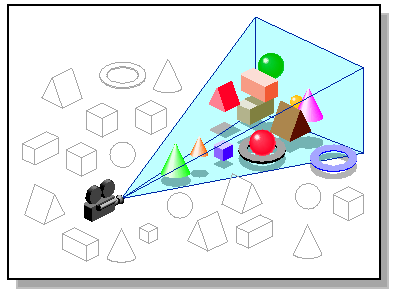
\includegraphics[width=\textwidth]{images/frustum_culling.png}
  \caption{Frustum Culling \cite{frustum_culling}}
  \label{fig:frustum_culling}
\end{figure}


This technique significantly improves performance as each object in the world is
contained within a ``bounding box'' which is often a cube or a sphere
\ref{fig:bounding_boxes}. Then for each object, a check is performed against the
bounded box instead of the actual vertices. This allow for in the best case a
single check or at its worst 8 checks per object. This is far better than
needing to perform thousands of checks for all the vertices of an object.

\begin{figure}[h!]
  \centering
  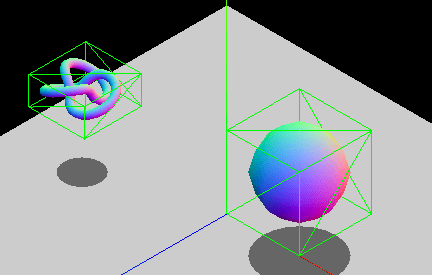
\includegraphics[width=\textwidth]{images/bounding_boxes.png}
  \caption{Bounding Boxes \cite{bounding_boxes}}
  \label{fig:bounding_boxes}
\end{figure}


\subsubsection{Spatial Acceleration Structures}
\gls{vmve} only supports loading basic models however, in the future many other
features need to be implemented. One such feature is large scale terrain as seen
in figure \ref{fig:quad_tree_terrain}.

\begin{figure}[h!]
  \centering
  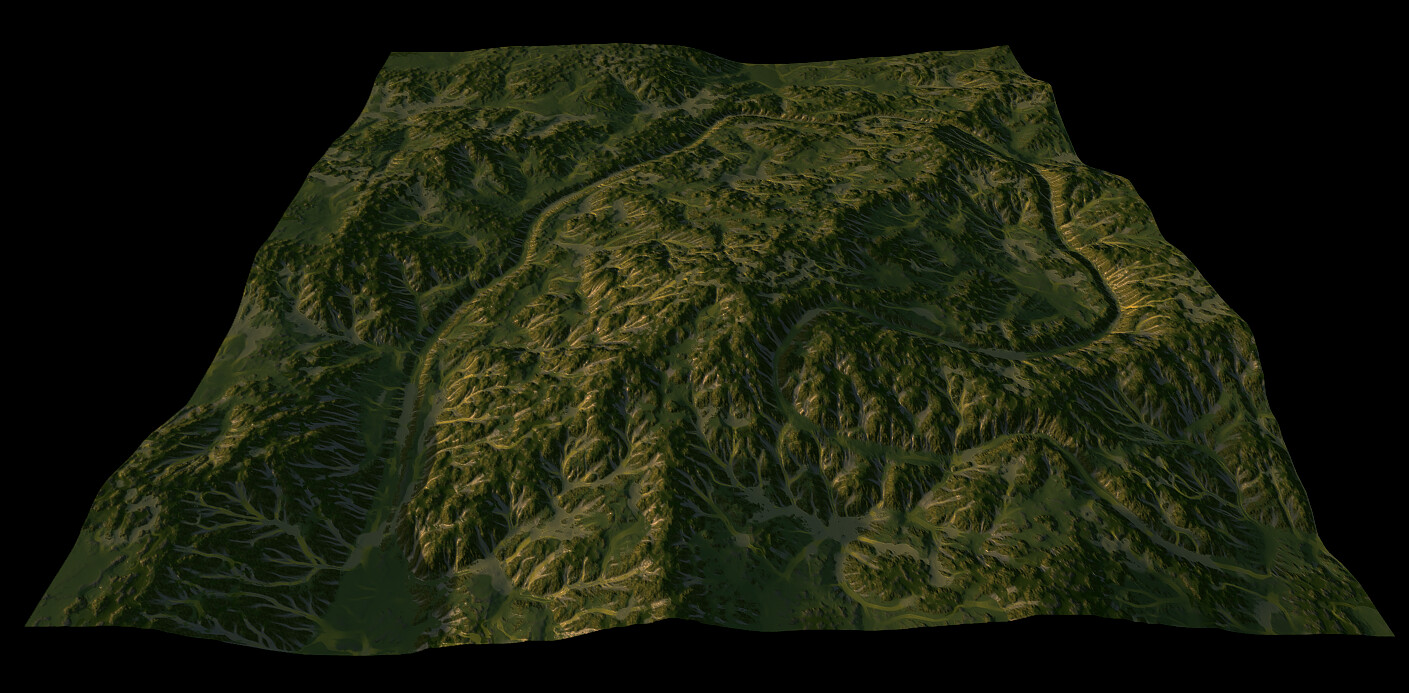
\includegraphics[width=\textwidth]{images/quad_tree_terrain.png}
  \caption{Large scale terrain}
  \label{fig:quad_tree_terrain}
\end{figure}

Currently, \gls{vmve} would struggle to render such objects due to its
complexity in terms of the number of vertices required. For example, an area of
20x20km with a resolution of 1 meter would require 400 million vertices. Each
vertex, if packed efficiently could be 32 bytes each that includes positions (12
bytes), normals (12 bytes) and texture coordinates (8 bytes). In terms of
memory, this would require 12.8GB of data just for the terrain.

A common solution to this, is implementing a type of spatial acceleration
structure also known as \gls{lod}. These structures are designed as the name
suggests, to increase the speed for algorithms in the spatial domain including
images and environments.

A quad tree is a type of spatial acceleration structure which stores a
hierarchical collection of nodes that each represent a 2D area (and an octree in
the case of 3D). Figure \ref{fig:quad_tree} visualizes a quad tree that shows
the resolution of each tile and how there are fewer tiles the further away from
the camera they are.

\begin{figure}[h!]
  \centering
  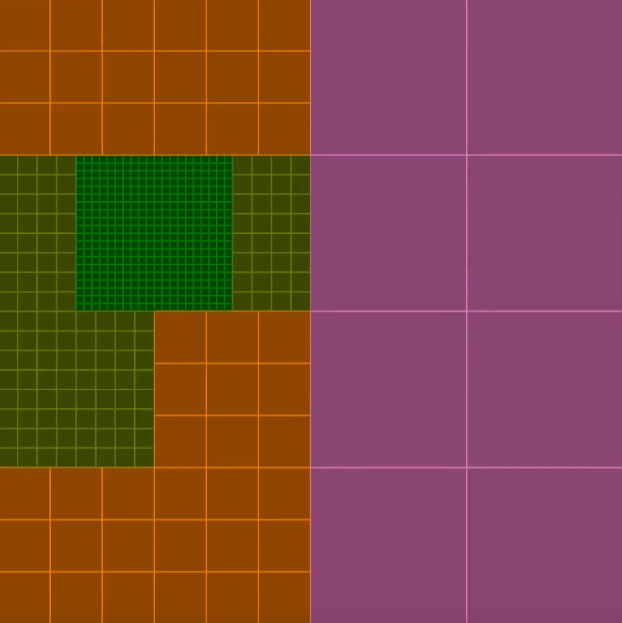
\includegraphics[width=\textwidth]{images/quad_tree.png}
  \caption{Quad Tree visualization}
  \label{fig:quad_tree}
\end{figure}

The benefit of using this technique is that the number of vertices are
significantly reduced saving on performance and memory usage.


\subsubsection{glTF Support}
Currently, the engine only really supports the VMVE and OBJ model formats for
importing. The main issue with the OBJ file format is its size since the data is
stored in a text format which subsequently increases the assets file size. glTF
\cite{gltf} is a new model format by The Khronos Group that has many useful
features such as compression, binary representation, scene hierarchy and more.

\subsection{Cross Platform}
Windows is the only operating system that \gls{vmve} officially supports.
Implementing cross platform support would greatly benefit the application as it
would increase flexibility in terms of which systems its able to run on and
subsequently, increase the potential user base. Implementing such functionality
would require significant changes to the underlying architecture of the
application such as implementing opaque types for structures that have a
different implementation depending on the operating system being used.

Additionally, a different build system has to be used that is cross platform.
The most commonly used cross platform build system is CMake \cite{cmake}.

\subsection{Networking Support}
VMVE is a virtual environment editor and as such can be significantly improved
by adding support for networking. The ideas is that there would be a server
running which would keep track of the virtual world and multiple clients via
VMVE would be able to connect and interact with the environment simultaneously.

This would allow for greater efficiency and speed up various tasks.

\subsection{Encryption}
VMVE supports both AES and Diffie-Helm encryption algorithms out of the box.
Additional work should be carried out to add more algorithms such as.....

\subsection{Version Control}
In regards to the VCS (version control system) architecture, a potential change
that can be done is to add a third branch called ``Beta''. The purpose of this
branch would be release relatively stable but yet unfinished features to users.
This would allow user to use new features and test them before an official
version is released. Overall this would reduce the number of bugs in final
versions and be beneficial to users who are keen in using recently developed
features. Figure \ref{fig:futurebrancharch} shows how the VCS architecture could
look like with the addition of a ``Beta'' branch.

\begin{figure}[h!]
  \centering
  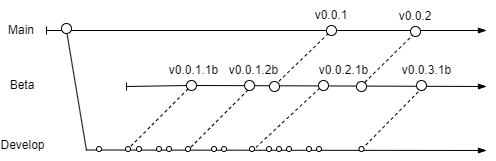
\includegraphics[width=\textwidth]{images/future_branch_design.png}
  \caption{Potential future git branch design}
  \label{fig:futurebrancharch}
\end{figure}

\subsection{Reduce library dependencies}
\gls{vmve} makes use of several libraries which allows specific functionality to be
added quickly. This is ideal given the projects time constrains and
requirements. However, going forward the aim will be to reduce the number of
external libraries being used.

This will provide various benefits such as less reliance of external code and
therefore, more control, smaller 


-- Replace libraries with a custom solution --
Lower footprint as only the required features are implemented.

\subsection{Accessibility}
Another aspect that needs to be addressed in the near future is improved
accessibility. The application includes some features that addresses this such
as icons, a tutorial, documentation as well as additional information. However,
some of the features that \gls{vmve} does not include is taking into account
color blindness and text to speech. The reason for this is that these are more
complex topics and required additional time and research to ensure a proper 
implementation is released.

Another task that must be considered is localization. \gls{vmve} only supports
the English language and has no way of adapting to other languages. Therefore,
the internal structure of the application must be redesigned to allow for
other languages to be added and thus, improving accessibility.

\section{Conclusion}

\gls{vmve} has been designed to be a platform in which users are provided easy to use
3D graphics tools without needing to know the complex details that come with
that. This allows users to worry less about technicalities and more about their
specific needs and requirements when using \gls{vmve}.

This has been a long journey that has presented me with various challenges
throughout the development of \gls{vmve}.


\clearpage
\printglossary

\clearpage
\printglossary[type=\acronymtype]


\bibliographystyle{IEEEtran}
\bibliography{refs}


\section{Appendices}
\begin{figure}[ht]
  \centering
  \begin{lstlisting}[language=C++]
    // Construct M (model)
    glm::mat4 m = glm::mat4(1.0f);
    m = glm::translate(m, world_position);   
    m = glm::rotate(m, radians, rotation_axis); 
    m = glm::scale(m, scale_amount);

    // Construct V (view)
    glm::mat4 v = glm::lookAt(camera_position, camera_direction, camera_up);

    // Construct P (projection)
    glm::mat4 p = glm::perspective(field_of_view, aspect_ratio, near, far);

    // Construct MVP
    glm::mat4 mvp = p * v * m; // Order is important

  \end{lstlisting}
  \caption{Complete MVP example}
  \label{fig:local_to_world_appendix}
\end{figure}


\end{document}

% end of document